%=======================================================================
%  Dinâmica inflacionária brasileira: choques de commodities,
%  inflação importada e o papel do câmbio
%  Enzo De Martino da Rocha — PUC-Rio
%
%  VERSÃO REVISADA. Alterações principais:
%   [1] Chaves de citação unificadas (elimina os "??" do PDF anterior)
%   [2] Referências corrigidas: stockl2017 (era "neto2015"),
%       carrarabarros2019 (era "carrara2015"), nogueirajr2007
%   [3] Período amostral uniformizado: 2003:01–2026:05
%   [4] Inflação importada incluída no vetor (sistema de 7 variáveis)
%   [5] Erro de sinal corrigido na hipótese de simetria (eq. lp)
%   [6] Definição de beta_n corrigida na Seção 2.1
%   [7] Rótulo duplicado "sec:naolinear" desfeito
%   [8] Labels ausentes criados; referências cruzadas manuais → \ref
%   [9] booktabs/amsmath carregados; Quadro 3.1 em ambiente quadroabnt
%  [10] abnt-etal-cite=3 (et al. só a partir de 4 autores)
%
%
%  ---------------------------------------------------------------------
%  REVISÃO 2 — correções aplicadas nesta versão:
%   [11] Chaves de citação do Cap. 3 corrigidas: carrara2019 ->
%        carrarabarros2019; nogueira2007 -> nogueirajr2007
%   [12] \label{cap:dados} criado (5 referências apontavam para o vazio)
%   [13] \ref{ape:robustez} -> \ref{ape:robustez} (4 ocorrências)
%   [14] Labels criados: sec:variaveis, sec:fri, sec:decomphist, sec:regime
%   [15] Seção 3.5.3 reposta (amortecimento x aversão a risco). O Cap. 1 e o
%        Cap. 2 prometiam esse exercício, que não constava do Cap. 3.
%   [16] Período amostral uniformizado de fato: maio/2026 no Resumo,
%        Abstract, Cap. 1 e Cap. 2 (antes diziam março)
%   [17] \textual inserido antes do Cap. 1 (faltava; quebrava a paginação)
%   [18] Quadro 3.1 movido para o ambiente quadroabnt; tabelas numeradas por
%        capítulo (\counterwithin), gerando Quadro 3.1 / Tabela 3.1 / Tabela A.1
%   [19] \paragraph -> \subsubsection na Seção 3.1.2, restaurando a
%        numeração 3.1.2.1–3.1.2.6 e limpando o sumário
%   [20] "definido em~(2.1)" -> \eqref{eq:erpt}; referências manuais de
%        seção do Cap. 3 trocadas por \ref
%   [21] \providecommand{\newlinetospace}: versões recentes do memoir
%        removeram esse comando, o que quebra o cabeçalho fora do Overleaf
%   [22] Lista do Apêndice A atualizada (sem Zivot-Andrews e sem Hamilton)
%   [23] Travessões eliminados do texto (72 ocorrências). Cada um foi
%        substituído conforme a função que exercia na frase: vírgula em
%        apostos curtos, parênteses quando o inciso já continha vírgulas,
%        dois-pontos quando introduzia explicação ou lista, e divisão em
%        nova frase nos casos mais longos. Os hifens duplos de intervalo
%        (2003:02--2026:05) foram preservados, pois são o uso correto.
%   [24] Ajuste sazonal do IPCA simplificado: fatores por variáveis binárias
%        de mês, estimados até 2019, no lugar do X-13ARIMA-SEATS. O IBC-Br
%        não é mais reajustado, pois o SGS 24364 já é dessazonalizado.
%        Efeito na Tabela 3.1: IPCA passa de ADF -9,27 / KPSS 0,07 para
%        ADF -10,01 / KPSS 0,09. A conclusão I(0) não muda.
%   [25] Seção 3.3.1: os três critérios de informação passam a indicar duas
%        defasagens (antes o AIC indicava três). A ordem escolhida segue
%        sendo p = 5, pela ausência de autocorrelação residual.
%   [26] Tabela A.1 recalculada na amostra em nível (2003:01--2026:05).
%  ---------------------------------------------------------------------
%  REVISÃO 3 — alinhamento ao material do curso (Econometria II, PUC-Rio):
%   [29] Capítulo 3 reescrito por inteiro seguindo os procedimentos e a
%        notação das aulas. Estimação e análise passam a ser feitas com o
%        pacote vars (VARselect, VAR, roots, stability, serial.test,
%        causality, irf, fevd), como na aula prática 14.
%   [30] Testes de raiz unitária: apenas ADF (ur.df), único teste
%        desenvolvido no curso. O KPSS foi retirado: aparece uma única vez
%        no material, citado numa lista de "outros testes".
%   [31] Pelo ADF no padrão do professor, a Selic NÃO rejeita a raiz
%        unitária em nenhuma especificação e passa a entrar em primeira
%        diferença. Isso elimina a discussão anterior de "I(0) persistente".
%   [32] Dessazonalização volta a ser X-13ARIMA-SEATS (seasonal::seas),
%        como na aula 10. O ajuste por variáveis binárias foi descartado.
%   [33] Exercício contrafactual removido: não consta do curso. O papel do
%        câmbio passa a ser medido pelo produto de duas funções de resposta
%        (Seção 3.4.2), que reproduz o mesmo número.
%   [34] Removido o exercício de regime de aversão a risco, que dependia do
%        contrafactual. As promessas correspondentes saíram do Cap. 1 e 2.
%   [35] Ordem de defasagens p = 5, pelo teste de Breusch-Godfrey.
%   [36] Capítulo 2 revisado por inteiro. Correções:
%        (a) a Seção 2.3.3 prometia que o Cap. 3 testaria o amortecimento
%            "em momentos de forte aversão a risco global"; esse exercício
%            foi removido, e a promessa foi reescrita.
%        (b) o parágrafo sobre grau de abertura estava solto dentro da
%            subseção de credibilidade; virou a Seção 2.2.2.
%        (c) a Seção 2.2.4 apresentava três não-linearidades sem dizer
%            quais seriam testadas; agora diz, e justifica a exclusão da
%            terceira.
%        (d) linguagem de método simplificada: "Curva de Phillips com
%            limiar" e "vetor autorregressivo com correção de erros"
%            passaram a ser descritos em palavras.
%        (e) retirada a generalização sem fonte sobre "os trabalhos sobre
%            o episódio" na antiga Seção 2.5.
%        (f) nova Seção 2.6, que reúne as decisões do Cap. 3 que decorrem
%            da revisão, dando fecho ao capítulo.
%   [37] Capítulo 1 reescrito. Correções:
%        (a) prometia medir o papel dual do câmbio "amplificador em fases
%            de depreciação, amortecedor em fases de apreciação", exercício
%            que foi retirado do Cap. 3; agora descreve o que o trabalho
%            de fato mede.
%        (b) retirada a promessa de "fornecer base empírica para a
%            calibração da função de reação do Banco Central", que o
%            trabalho não entrega.
%        (c) registro simplificado: frases mais curtas, menos subordinadas,
%            sem a oposição "ponto de vista positivo x normativo".
%        (d) a pergunta de pesquisa passou a incluir explicitamente o papel
%            do câmbio, que é o objetivo central declarado no Cap. 3.
%   [38] Resumo e Abstract alinhados ao Cap. 3: sai a promessa do papel
%        dual por regime cambial, entra a descrição do que é estimado.
%        "VAR/SVAR" passa a "vetores autorregressivos" e a palavra-chave
%        SVAR passa a VAR, já que a identificação é por Cholesky simples.
%  ---------------------------------------------------------------------
%   [27] Carta Aberta de 2021 conferida na fonte: os 4,38 p.p. de inflação
%        importada sobre um desvio de 6,31 p.p. estão CORRETOS. A soma de
%        petróleo, commodities e câmbio (4,10 p.p.) não fechava porque a
%        rubrica tem componentes adicionais. A decomposição completa foi
%        acrescentada em nota de rodapé na Introdução.
%   [28] Capítulo 2 reescrito por inteiro em registro de graduação. Retirada
%        a Seção 2.5 antiga (revisão da literatura internacional pós-2021,
%        com a controvérsia oferta x demanda e a crítica metodológica de
%        Bergholt), substituída por uma seção curta sobre o choque de
%        2021-2022. Saíram as citações arce2024, ascari2024, bergholt2024,
%        gopinath2020 e lansing2026. O capítulo caiu de 19 para 8 páginas.
%        Corrigida, com isso, a promessa quebrada da antiga Seção 2.5.4,
%        que dizia incorporar à Seção 3.4.2 duas correções que o Capítulo 3
%        não implementava.
%  ---------------------------------------------------------------------
%
%  Nao ha pendencias de bibliografia: o Capitulo 3 passou a usar apenas o
%  teste ADF, e a entrada kwiatkowski1992 deixou de ser citada.
%
%  Todos os marcadores [VERIFICAR] foram resolvidos (ver itens [27] e [28]).
%=======================================================================
%
%  REVISÃO 4 — Seção 3.4.2 refeita a pedido do orientador:
%
%   [39] A medida do papel do câmbio deixou de ser o produto de duas
%        respostas acumuladas (A_n = -theta x beta) e passou a ser a
%        diferença entre a FRI usual e uma FRI contrafactual em que o
%        câmbio é mantido na trajetória de base por inovações
%        compensatórias período a período. É o procedimento de Sims e
%        Zha, aplicado por Bernanke, Gertler e Watson (1997, p. 106).
%        Motivo: o produto das duas respostas ignora as realimentações
%        do sistema, e a resposta total já contém o movimento do câmbio
%        dentro dela. Duas referências novas: simszha2006, bernanke1997.
%        A limitação correspondente, no fim do Capítulo 3, foi reescrita.
%
%   [40] Capítulo 4 (Resultados) escrito. Cinco seções: diagnósticos,
%        respostas a impulso (Tabela 4.1), canal do câmbio (Tabela 4.2 e
%        Figura 4.1), decomposição da variância e Granger (Tabela 4.3),
%        estabilidade (Tabelas 4.4 e 4.5) e síntese. Todos os números
%        vêm das saídas do 02_var.R, em Tabs/. Pacote multirow carregado
%        para a Tabela 4.1. A figura usa graficos/07_contrafactual.pdf.
%
%  REVISÃO 5 — revisão geral do PDF (capítulos 1 a 4):
%
%   [41] Resumo e Abstract reescritos: saíram do tempo futuro e passaram a
%        reportar os resultados (0,078 / 0,102 / 0,133 / 0,055 p.p.).
%   [42] Seção 4.2: retirada a afirmação de que a magnitude estaria "na faixa
%        que a literatura brasileira recente encontra", que remetia a uma
%        seção sem números de comparação. Substituída por remissão à
%        Seção 2.4.2, que de fato sustenta a leitura.
%   [43] Seção 3.4.3: horizontes da decomposição da variância corrigidos de
%        "3, 6, 12 e 24" para "3, 12 e 24", que é o que a Tabela 4.3 traz.
%   [44] Seção 3.1.3: "choque de 2020 e 2021" corrigido para "2021 e 2022".
%   [45] Seção 2.4.3: descrição do método atualizada. Não é mais medição
%        direta a partir das FRIs, e sim contrafactual sobre o sistema já
%        estimado. Acrescentado o contraste com Stöckl et al., que reestimam
%        o sistema sem o câmbio.
%   [46] Numeração das figuras por capítulo (\counterwithin{figure}{chapter}).
%   [47] Data da capa: agosto -> setembro de 2026.
%   [48] Seção 4.4: acrescentado parágrafo explicando por que a ordem da
%        decomposição da variância difere da ordem da Tabela 4.1 (efeito por
%        unidade x ponderação pela volatilidade de cada choque).
%   [49] Seção 4.3: "quase o dobro" -> "cerca de setenta por cento acima"
%        (0,133/0,078 = 1,7).
%   [50] Seção 3.3.1: réplicas do bootstrap especificadas (mil no sistema
%        completo, quinhentas nos exercícios com reestimação).
%   [51] "pouco menos de trinta por cento" e "pouco menos de um terço"
%        harmonizados em "cerca de trinta por cento" (o número é 29,0%).
%
%
%  REVISÃO 6 — simplificação de linguagem (sem mudar nenhum resultado):
%
%   [52] Seção 2.2.4: os três padrões de não-linearidade viraram três
%        parágrafos curtos (sinal, tamanho, momento), em vez de um bloco
%        único com "o primeiro / o segundo / o terceiro".
%   [53] Seção 2.6: reescrita em frases mais curtas; a abertura deixou de
%        ser "Convém encerrar reunindo as decisões que a revisão sugere".
%   [54] Seção 3.3.2: o parágrafo com seis justificativas de ordenação foi
%        quebrado em três, um por bloco de variáveis.
%   [55] Seção 3.4.2: as três decisões de implementação viraram três
%        parágrafos, cada um respondendo a uma pergunta clara.
%
%
%  REVISÃO 7 — passada geral de linguagem (nenhum resultado alterado):
%
%   [56] Retiradas as aberturas de parágrafo formais e vazias: "Convém
%        notar", "Cabe registrar", "Vale registrar", "devem ser reconhecidas
%        de antemão", "Há, porém, uma qualificação importante".
%   [57] Frases acima de 40 palavras quebradas em duas ou três, no Resumo,
%        no Abstract, nas Seções 2.2.3, 2.4.3, 3.1.2.2, 4.5.1 e na abertura
%        do Capítulo 4.
%   [58] Introdução: "o Capítulo 4" passou a usar \ref{cap:resultados}.
%
%
%  REVISÃO 12 — comentários do orientador na versão preliminar:
%
%   [71] CORREÇÃO DE MÉTODO, a mais importante. O repasse deixou de ser a
%        resposta acumulada do IPCA dividida pelo impacto inicial do
%        choque e passou a ser a divisão pela variação ACUMULADA da
%        variável de origem no mesmo horizonte (nova equação 3.6). Motivo
%        dado pelo orientador: a variável continua respondendo ao choque
%        depois do primeiro mês, e é a variação acumulada dela que importa
%        para a variação acumulada do nível de preços. Muda as Tabelas
%        4.1, 4.2 e 4.4, o Resumo, o Abstract e a Síntese. Em 12 meses:
%        commodities 0,078 -> 0,059; câmbio 0,102 -> 0,079; contrafactual
%        0,133 -> 0,101; canal cambial -0,055 -> -0,042. O intervalo de
%        confiança passou a vir de bootstrap da própria razão, e não das
%        bandas do numerador, que ignoravam a incerteza do denominador.
%   [72] Acrescentadas as Figuras 4.1 e 4.2, com as respostas do IPCA
%        pontuais e acumuladas, antes da Tabela 4.1, a pedido dele.
%   [73] Causalidade de Granger passou a ter tabela própria (Tabela 4.4),
%        com estatística F, graus de liberdade e valor-p. Antes o texto
%        descrevia o resultado sem mostrar número.
%   [74] Nova Seção 4.6: robustez da ordenação de Cholesky, com o modelo
%        reestimado sob três ordens alternativas (Tabela 4.7). Os
%        resultados praticamente não se movem.
%   [75] Seção 3.1.2.2: acrescentados o gráfico comparativo IC-Br x preços
%        de importação (Figura 3.1) e as correlações, 0,87 em nível e
%        0,25 em variação mensal.
%   [76] Seção 3.1.2.1: registrada a endogeneidade parcial do IC-Br, cujos
%        pesos foram construídos a partir da relevância de cada commodity
%        para a inflação brasileira. Vira também a quinta limitação.
%   [77] Seção 3.6: sexta limitação, sobre o VAR com exogeneidade em
%        bloco. A ordenação impede efeito contemporâneo das domésticas
%        sobre as externas, mas não zera as defasagens.
%   [78] Seção 2.1: título passou a "O repasse do câmbio e dos preços
%        externos" e o escopo do conceito ficou explícito, distinguindo
%        repasse cambial de repasse de preços externos.
%   [79] Seção 2.6: a justificativa para incluir hiato e Selic foi
%        reordenada. A razão principal é entender os canais de
%        transmissão; a ajuda na identificação é secundária.
%   [80] Seção 2.6: o fecho deixou de apresentar o contrafactual como
%        única contribuição e passou a listar as três.
%   [81] Seção 3.3.2: retirada a menção em terceira pessoa ao julgamento
%        do pesquisador e acrescentado que a ordenação é necessariamente
%        arbitrária, com remissão ao exercício de robustez.
%   [82] Seções 3.5.1 e 4.5.1: explicitado que comparar intervalos não é
%        teste formal, e sim evidência indicativa.
%   [83] Seções 3.5.2 e 4.5.2: explicitado que a regressão de assimetria é
%        ilustrativa e trata o câmbio como exógeno, ao contrário do VAR.
%
%   [84] COMENTARIO QUE EU TINHA PERDIDO: na primeira leitura das
%        anotacoes do PDF a extracao falhou antes da ultima pagina e o
%        comentario da p.38 nao apareceu. Ele pedia uma secao comparando
%        os resultados com a literatura, alem da conclusao. Secao 4.7
%        escrita (Como esses resultados se comparam a literatura). A
%        conclusao fica para o Capitulo 5, na versao final.
%   [85] Secao 3.1.2.5: a justificativa da Selic ainda dizia que sem ela a
%        resposta "viria contaminada". O orientador havia corrigido isso
%        (p.22, "nao necessariamente - veja comentario mais acima"). A
%        razao principal passou a ser a mesma da Secao 2.6: a reacao do
%        Banco Central faz parte do mecanismo que se quer entender.
%   [86] Secao 2.6: "a Secao 2.2.4 mostrou" -> "sugere", como ele anotou.
%   [87] Introducao: acrescentado paragrafo deixando explicito que o
%        episodio de 2021 e 2022 e o centro do interesse, o que ele
%        observou nao estar claro na motivacao (p.23).
%
%   [88] Secao 2.1: a definicao de beta_n foi corrigida na origem. A
%        equacao (2.1) passou a ter denominador acumulado, e caiu a frase
%        que dizia que as FRIs acumuladas "podem ser lidas diretamente
%        como estimativa de beta_n", que era justamente o erro apontado
%        pelo orientador na p.10. Acrescentado o paragrafo explicando por
%        que o denominador precisa acumular.
%
%   [89] Abertura do Capitulo 4 atualizada: listava quatro secoes e o
%        capitulo passou a ter seis, com a robustez da ordenacao e a
%        comparacao com a literatura.
%
%  REVISÃO 13 — passada final de registro (nenhum numero alterado):
%
%   [90] Reduzidas de 27 para 10 as enumeracoes do tipo "A primeira e / A
%        segunda e / A terceira e", que davam ao texto um ritmo mecanico.
%        Afetou as Secoes 2.6, 3.3.2, 3.4.2, 4.1, 4.3, 4.5.1 e 4.7.
%   [91] Afirmacoes categoricas suavizadas: "O resultado confirma o
%        mecanismo" -> "vai na direcao esperada"; "Os resultados sao
%        claros" retirado; "onde mora o erro mais comum" -> "merece
%        atencao"; "coerente com o consenso da literatura" -> "com o que a
%        literatura vinha encontrando"; "a diferenca provavel" -> "uma
%        explicacao possivel"; "ja captam o que havia para captar" ->
%        "parecem captar o que ha para captar".
%   [92] Variadas as aberturas repetidas ("Falta dizer", "Falta explicar",
%        "Tres leituras se destacam").
%
%   [93] O item [87] foi desfeito. Em vez de acrescentar um paragrafo a
%        introducao afirmando que o choque de 2021-22 e o objeto central,
%        a frase da Secao 3.1.3 foi rebaixada: o choque "esta no centro do
%        periodo que se quer medir". Some a afirmacao forte, sem deixar a
%        escolha de manter o periodo pandemico sem justificativa.
%
%   PENDENTE (dados): o orientador sugeriu duas verificações que dependem
%   de séries que ainda não estão no painel. (a) refazer o exercício com
%   um índice internacional de commodities cujos pesos não dependam da
%   inflação brasileira; (b) um teste de robustez incluindo as
%   expectativas de inflação do Boletim Focus.
%
%   PENDENTE (fora do .tex): no references.bib, a entrada nogueirajr2007 está
%   com o sobrenome em caixa alta e sai como "NOGUEIRA JÚNIOR (2007)" no corpo
%   do texto. Corrigir o campo author para {Nogueira Júnior, Reginaldo P.}.
%=======================================================================

\documentclass[12pt,openright,oneside,a4paper,portuguese,brazil]{abntex2}

% -- ESTRUTURA BÁSICA -- %
% abnt-etal-cite=3 / abnt-etal-list=3: "et al." apenas com MAIS de 3 autores,
% conforme NBR 6023:2018 (8.1.1.2). Antes estava em 2, o que gerava
% "Sims et al. (1990)" para três autores — erro de norma.
\usepackage[alf,abnt-etal-cite=3,abnt-etal-list=3]{abntex2cite}
\usepackage[a4paper,margin=3cm]{geometry}
\usepackage{caption}

% -- MATEMÁTICA E TABELAS -- %
\usepackage{amsmath}
\usepackage{amssymb}
\usepackage{booktabs}          % \toprule \midrule \bottomrule
\usepackage{multirow}          % células que ocupam várias linhas (Tabela 4.1)
\usepackage[flushleft]{threeparttable}
\usepackage{float}
% Float próprio para quadros (NBR 14724 / IBGE): título acima, fonte abaixo.
\newfloat{quadroabnt}{htbp}{loq}[chapter]
\floatname{quadroabnt}{Quadro}
% Numeracao de tabelas por capitulo (3.1, 3.2...), para ficar
% coerente com a numeracao dos quadros.
\counterwithin{table}{chapter}
\counterwithin{figure}{chapter}

% -- ESTÉTICA -- %
\usepackage{fancyhdr}
\pagestyle{fancy}
% Fallback: \newlinetospace foi removido de versoes recentes do memoir.
% Sem isto, o cabecalho quebra em distribuicoes TeX Live mais novas.
\providecommand{\newlinetospace}[1]{#1}

% Profundidade de numeração e de sumário: impede que \paragraph gere
% entradas do tipo "3.1.2.0.1" no sumário (violação da NBR 6024).
\setcounter{secnumdepth}{3}
\setcounter{tocdepth}{3}

%% -- SUMÁRIO -- %%
\cftsetindents{chapter}{3em}{2em}
\cftsetindents{section}{5em}{2em}
\cftsetindents{subsection}{5em}{3em}

% -- MARGENS -- %
\usepackage{ragged2e}
\usepackage{enumitem}
\setlist[itemize]{leftmargin=1.5em, labelsep=0.5em, itemsep=0.5em}

% -- FONTES E TÍTULOS -- %
\usepackage{titlesec}

\titleformat{\chapter}[hang]
  {\sffamily\bfseries\Large}{\thechapter}{8pt}{\Large\raggedright}
\titlespacing*{\chapter}{0pt}{-50pt}{40pt}

\titleformat{\section}
  {\sffamily\bfseries\large}{\thesection}{8pt}{}

\titleformat{\subsection}
  {\sffamily\bfseries\normalsize}{\thesubsection}{1em}{}
% Sem esta linha, as subsubseções (3.1.2.1 etc.) saem em fonte serifada,
% destoando de todos os demais títulos, que são sans-serif.
\titleformat{\subsubsection}
  {\sffamily\bfseries\normalsize}{\thesubsubsection}{1em}{}

\usepackage{graphicx}
\graphicspath{{./}{graficos/}{figuras/}}  % procura as figuras na raiz e nessas pastas

% Metadados do PDF em texto literal: \@title e \@author não estão
% definidos neste documento e quebrariam a compilação.
\hypersetup{
  pdftitle={Dinâmica inflacionária brasileira: choques de commodities, inflação importada e o papel do câmbio},
  pdfauthor={Enzo De Martino da Rocha},
  pdfsubject={Monografia de Final de Curso},
  pdfkeywords={inflação, commodities, pass-through cambial, IPCA, VAR},
  pdfcreator={LaTeX with abnTeX2},
  colorlinks=true,
  linkcolor=black,
  citecolor=blue,
  urlcolor=blue
}

% Título do sumário
\makeatletter
\renewcommand{\tableofcontents}{%
  \chapter*{SUMÁRIO}
  \@starttoc{toc}
}
\makeatother


\begin{document}
% NBR 14724/6023: o elemento pós-textual denomina-se "Referências".
% Precisa vir DEPOIS de \begin{document}: o babel redefine \bibname na abertura.
\renewcommand{\bibname}{REFERÊNCIAS}
\setcounter{tocdepth}{3}
\pretextual
\selectlanguage{portuguese}

\setlength{\parskip}{10pt}

%=======================================================================
% FOLHA DE ROSTO
%=======================================================================
\pagenumbering{arabic}
\pagestyle{fancy}

\renewcommand{\chaptermark}[1]{\markboth{#1}{}}
\renewcommand{\sectionmark}[1]{\markright{#1}{}}

\fancyhf{}
\fancyhead[RO]{\textit{\nouppercase{\newlinetospace{{\leftmark}}}}}

\flushright
\thispagestyle{empty}
\includegraphics[width=10cm]{logo_puc.png}

\vspace{20pt}

\large{Enzo De Martino da Rocha}

\vspace{100pt}

\Large{\textbf{\sffamily Dinâmica inflacionária brasileira: choques de commodities, inflação importada e o papel do câmbio}}

\vspace{90pt}

\normalsize
Monografia de Final de Curso

\vspace{2pt}

Orientador: Marco Cavalcanti

\vspace{40pt}

\centering

Declaro que o presente trabalho é de minha autoria e que não recorri, para realizá-lo, a nenhuma forma de ajuda externa, exceto quando autorizado pelo professor tutor.

\vspace{60pt}

% A data precisa ser posterior ao término da amostra (maio de 2026).
Rio de Janeiro, setembro de 2026

\flushleft
\pagebreak


%=======================================================================
% AGRADECIMENTOS
%=======================================================================
\section*{Agradecimentos}
\justifying
\hspace{1em}

Agradeço à minha família, pelo apoio incondicional ao longo de
toda a minha trajetória acadêmica e pela confiança depositada em
mim em cada etapa deste percurso.

Ao professor Marco Cavalcanti, referência em Econometria, agradeço
por ter me ensinado os conceitos práticos que viabilizaram os
resultados deste trabalho e por sua participação decisiva no
direcionamento temático desta monografia.

Por último, mas não menos importante, a mim mesmo, pela
perseverança ao longo do curso e pelo empenho depositado na
conclusão deste trabalho.
\newpage


%=======================================================================
% RESUMO
%=======================================================================
\section*{Resumo}
\justifying
\hspace{1em}
O presente trabalho investiga a dinâmica inflacionária brasileira recente,
com ênfase na contribuição relativa dos choques internacionais de
commodities, da inflação importada e da taxa de câmbio na determinação
do Índice Nacional de Preços ao Consumidor Amplo (IPCA). A estratégia
empírica baseia-se na estimação de um modelo de vetores autorregressivos com
séries mensais de janeiro de 2003 a maio de 2026, do qual se obtêm funções de
resposta a impulso e a decomposição da variância. A análise é complementada por
dois exercícios que verificam se o repasse cambial mudou ao longo do tempo e se
difere entre depreciações e apreciações. A hipótese central é a de que os preços internacionais de commodities são um
determinante relevante da inflação doméstica. A taxa de câmbio, por sua vez,
cumpre papel duplo: repassa parte do choque aos preços e ao mesmo tempo o
amortece, porque a alta das cotações internacionais tende a apreciar o real.
Os resultados sustentam essa hipótese. Uma variação acumulada de 1\% nos
preços de commodities eleva o nível de preços em 0,059\% ao fim de doze meses,
e uma variação cambial de mesma magnitude o eleva em 0,079\%. Um exercício
contrafactual, em que a taxa de câmbio é impedida de responder ao choque de
commodities, mostra que o efeito seria de 0,101\% na ausência da resposta
cambial: a apreciação do real absorve 0,042 ponto percentual. Os preços de
importação, uma vez controlados os dois primeiros canais, não apresentam
efeito estatisticamente distinto de zero.

\vspace{\onelineskip}
% NBR 6028: recomendam-se de três a cinco palavras-chave.
\noindent\textbf{Palavras-chave}: inflação. commodities. pass-through
cambial. IPCA. VAR.

\newpage

%=======================================================================
% ABSTRACT
%=======================================================================
\section*{Abstract}
\begin{otherlanguage*}{english}
\justifying
\hspace{1em}
This paper investigates recent Brazilian inflationary dynamics, with
emphasis on the relative contribution of international commodity shocks,
imported inflation and the exchange rate to the determination of the
Consumer Price Index (IPCA). The empirical strategy is based on the
estimation of a vector autoregression using monthly data from January 2003 to
May 2026, from which impulse response functions and the forecast error variance
decomposition are obtained. The analysis is complemented by two exercises that
assess whether exchange rate pass-through has changed over time and whether it
differs between depreciations and appreciations. The central hypothesis is that international commodity prices are a relevant
determinant of domestic inflation. The exchange rate, in turn, plays a dual
role: it passes part of the shock through to prices while also dampening it,
because rising international commodity prices tend to appreciate the domestic
currency. The results support this hypothesis. A 1\% cumulative increase in
commodity prices raises the price level by 0.059\% after twelve months, while
an exchange rate movement of the same size raises it by 0.079\%. A
counterfactual exercise, in which the exchange rate is prevented from
responding to the commodity shock, shows that the effect would reach 0.101\%
in the absence of the exchange rate response: the appreciation of the real
absorbs 0.042 percentage point. Import prices, once the first two channels are
controlled for, show no effect statistically different from zero.

\vspace{\onelineskip}
\noindent\textbf{Keywords}: inflation. commodities. exchange rate
pass-through. IPCA. VAR.
\end{otherlanguage*}


%=======================================================================
% SUMÁRIO
%=======================================================================
\sffamily
\tableofcontents

\rmfamily


%=======================================================================
\textual

\chapter{Introdução}
\label{cap:introducao}
\justifying

O controle da inflação é um tema central da política econômica brasileira. Da
alta inflação crônica que perdurou até o Plano Real, em 1994, à consolidação do
regime de metas em 1999, a estabilidade de preços tornou-se o principal
compromisso da política monetária no país. Entender quais fatores explicam a inflação recente ajuda de duas formas.
Primeiro, a compreender o comportamento dos preços. Segundo, a discutir como a
política monetária deve reagir a choques vindos de fora.

Ao longo das décadas de 1980 e início de 1990, o Brasil enfrentou cinco planos
de estabilização fracassados, do Cruzado ao Collor, todos incapazes de romper a
inércia inflacionária \cite{giambiagi2011}. Foi apenas com o Plano Real que o
país conseguiu estabilizar os preços de forma duradoura.

A adoção do regime de metas de inflação em 1999, ao lado do câmbio flutuante e
da responsabilidade fiscal, consolidou o arcabouço que orienta a atuação do
Banco Central até hoje. \citeonline{minella2003} destacam que um banco central
comprometido com metas anunciadas de antemão ajuda a coordenar as expectativas
dos agentes, o que contribui para um cenário inflacionário mais estável.

Ainda assim, a estabilidade não tornou o país imune a choques. A crise fiscal e
cambial de 2015 e 2016 levou o IPCA a patamares próximos de dez por cento, os
maiores desde 2002 \cite{ibge_ipca}. Mais recentemente, o choque de 2021 e 2022,
agravado pela desorganização das cadeias globais de suprimento e pela guerra na
Ucrânia, recolocou o tema no centro do debate. O descumprimento das metas levou
o Banco Central a enviar Cartas Abertas em 2021, 2022 e 2024, atribuindo parcela
importante do desvio à combinação de choques de commodities, depreciação cambial
e inflação importada. Em 2021, quando o IPCA fechou em 10,06\% contra meta de
3,75\%, a inflação importada respondeu por 4,38 p.p.\ do desvio total de 6,31
p.p.\ \cite{bcb2022carta}.\footnote{Na decomposição apresentada pela autoridade
monetária, a inflação importada responde por cerca de 69\% do desvio, sendo os
principais componentes o preço do petróleo (2,95 p.p.), os demais preços de
commodities medidos pelo IC-Br (0,71 p.p.) e a taxa de câmbio (0,44 p.p.). Os
demais fatores citados são a inércia do ano anterior (1,21 p.p.), a bandeira
tarifária de energia elétrica (0,67 p.p.) e as expectativas de inflação (0,25
p.p.), parcialmente compensados pelo hiato do produto negativo ($-1{,}21$
p.p.).}

Nesse quadro, o preço internacional de commodities aparece como um dos
principais canais de transmissão de pressões inflacionárias para a economia
brasileira. O país exporta sobretudo produtos primários e depende de insumos
cotados em mercados internacionais, o que o deixa exposto a choques externos de
preços. Variações nas cotações de petróleo, grãos e metais elevam custos de
produção, pressionam a taxa de câmbio e chegam aos preços ao consumidor
\cite{carrarabarros2019}.

Para uma economia que ao mesmo tempo exporta e importa commodities, esse
mecanismo tem uma característica particular. A alta das cotações internacionais
pressiona os preços diretamente, mas também tende a apreciar o real, porque
melhora os termos de troca do país. A apreciação, por sua vez, reduz em reais a
mesma alta que pressionava os preços. O câmbio, portanto, transmite parte do
choque e ao mesmo tempo o amortece \cite{stockl2017}. Medir o tamanho desse
amortecimento é um dos objetivos deste trabalho.

A pergunta que orienta a monografia é, então: \textit{qual o peso relativo dos
choques de commodities, da inflação importada e da taxa de câmbio na dinâmica
recente do IPCA, e qual o papel do câmbio na transmissão desses choques?}

Para respondê-la, estima-se um modelo de vetores autorregressivos com séries
mensais entre janeiro de 2003 e maio de 2026. O modelo reúne o IPCA, a taxa de
câmbio, os preços internacionais de commodities, os preços de importação e
variáveis de controle da economia doméstica. A partir dele, calculam-se funções
de resposta a impulso e a decomposição da variância, que medem quanto cada
choque contribui para a inflação. A análise é complementada por dois exercícios
simples, que verificam se o repasse cambial mudou ao longo do tempo e se
depreciações e apreciações têm o mesmo efeito sobre os preços.

O trabalho pretende acrescentar uma medida atualizada desses efeitos, estimada
em amostra que cobre por inteiro o choque inflacionário de 2021 e 2022 e sua
dissipação, período ainda pouco coberto pelos trabalhos aplicados disponíveis
para o Brasil.

O trabalho está organizado da seguinte forma. O Capítulo~\ref{cap:revisao}
apresenta a revisão da literatura sobre inflação importada, choques de
commodities e pass-through cambial. O Capítulo~\ref{cap:dados} descreve os dados
e a estratégia empírica. O Capítulo~\ref{cap:resultados} discute os resultados
e o Capítulo~\ref{cap:conclusao} apresenta as conclusões.

\chapter{Inflação importada, choques de commodities e pass-through cambial: uma revisão da literatura}
\label{cap:revisao}

Este capítulo revisa a literatura sobre os canais que ligam choques externos à
inflação brasileira. A Seção~\ref{sec:erpt-def} define o conceito de repasse. A Seção~\ref{sec:determinantes} discute o que torna esse
repasse maior ou menor. A Seção~\ref{sec:commodities} descreve os caminhos
pelos quais choques de commodities chegam aos preços domésticos. A
Seção~\ref{sec:evidencia} resume a evidência empírica para o Brasil e a
Seção~\ref{sec:posspandemia} trata do choque inflacionário de 2021 e 2022. A Seção~\ref{sec:implicacoes} reúne o que essa revisão implica para a
estratégia empírica do Capítulo~\ref{cap:dados}.

\section{O repasse do câmbio e dos preços externos}
\label{sec:erpt-def}

O termo \textit{exchange rate pass-through} designa o grau em que variações na
taxa de câmbio nominal se transmitem aos preços em moeda doméstica.
\citeonline{goldberg1997} definem o conceito como a elasticidade dos preços
domésticos em relação à taxa de câmbio, mantidos constantes os demais
determinantes de preços.

Denotando por $P_t$ o nível de preços e por $E_t$ a taxa de câmbio nominal, o
repasse contemporâneo é $\beta_0 = \partial \ln P_t / \partial \ln E_t$. Como o
ajuste de preços não é imediato, a literatura reporta o repasse acumulado ao
longo de $n$ meses. Escrevendo $\Delta_n x$ para a variação acumulada de $x$
entre $t$ e $t+n$,

\begin{equation}
\beta_{n} \;=\; \frac{\Delta_n \ln P}{\Delta_n \ln E}
\;=\; \frac{\sum_{i=0}^{n} \pi_{t+i}}{\sum_{i=0}^{n} \Delta \ln E_{t+i}} ,
\label{eq:erpt}
\end{equation}

\noindent em que $\pi_{t} = \Delta \ln P_{t}$. Numerador e denominador são,
ambos, somas acumuladas até o mesmo horizonte.

O denominador merece atenção. Se a taxa de câmbio subisse uma única vez e
ficasse parada no novo patamar, a variação acumulada dela seria igual à do
primeiro mês, e bastaria somar as respostas da inflação para obter $\beta_n$. Não é o que acontece: depois de um
choque, o câmbio continua se movendo por vários meses. O denominador precisa,
portanto, acumular também. É essa a forma usada no Capítulo~\ref{cap:dados},
na equação~\eqref{eq:repasse}.

Um valor de $\beta_n$ próximo de um indica repasse completo; valores
intermediários indicam repasse parcial; e valores próximos de zero indicam
ausência de repasse.

Neste trabalho o conceito é usado em sentido mais amplo, e convém fixar a
terminologia desde já. \textit{Repasse cambial} designa o efeito de uma
variação da taxa de câmbio sobre os preços domésticos, que é o objeto clássico
da literatura. \textit{Repasse de preços externos} designa o efeito de uma
variação nas cotações internacionais medidas em dólar, seja de commodities,
seja dos bens importados. Quando o texto disser apenas repasse, sem
qualificação, trata-se do cambial.

Os dois andam juntos, porque o preço de importação em reais é o produto entre
a cotação internacional $P^{*}_{t}$ e a taxa de câmbio $E_{t}$. Separá-los é
útil, pois permite dizer quanto de um choque inflacionário veio do mercado
internacional e quanto veio da conversão cambial. Essa separação é um dos
objetivos do exercício empírico.

\citeonline{campa2005} distinguem dois estágios do repasse. O de primeiro
estágio mede quanto uma variação cambial afeta os preços de importação na
fronteira. O de segundo estágio mede quanto essa variação chega aos preços ao
consumidor. O segundo é sistematicamente menor que o primeiro, porque entre a
fronteira e a prateleira existem margens de comércio, custos de distribuição e
serviços que não são importados. A distinção importa para a leitura dos
resultados deste trabalho, que estima o repasse ao IPCA, ou seja, o de segundo
estágio.

Uma regularidade bem documentada é a queda do repasse nas economias
desenvolvidas a partir dos anos 1990. \citeonline{taylor2000} associa essa queda
ao ambiente de inflação baixa e estável do período: quando a inflação é baixa,
as firmas tratam choques de custo como temporários e ajustam menos os preços.
Essa hipótese organizou boa parte da literatura posterior.

\section{O que faz o repasse ser maior ou menor}
\label{sec:determinantes}

O coeficiente de repasse não é um número fixo. Ele depende de características da
economia e do momento em que é medido. Isso significa que estimativas obtidas em
outros países, ou em períodos distintos da história brasileira, não podem ser
transportadas sem cuidado. Esta seção reúne os fatores mais citados pela
literatura.

\subsection{Estrutura de mercado}
\label{sec:ptm}

Firmas exportadoras com poder de mercado nem sempre repassam integralmente uma
variação cambial. Elas podem absorver parte dela na margem de lucro, para manter
o preço estável no país de destino. Esse comportamento é chamado de
\textit{pricing-to-market} e foi formalizado por \citeonline{krugman1987} e
\citeonline{dornbusch1987}.

A intensidade do comportamento varia com o tipo de bem. Em mercados de bens
homogêneos, como as commodities agrícolas, metálicas e energéticas, a arbitragem
internacional impõe um preço único e o repasse é praticamente completo. Em bens
manufaturados diferenciados, com marca e canal de distribuição próprios, o
exportador tem mais espaço para ajustar margens, e o repasse é menor.

Essa diferença importa para o Brasil, cuja pauta importadora combina insumos
próximos de commodities, como combustíveis e fertilizantes, com manufaturados
diferenciados, como produtos químicos e bens de capital. É também a razão pela
qual o Capítulo~\ref{cap:dados} trata os preços de commodities e os preços de
importação como duas variáveis distintas, e não como uma só: espera-se que o
repasse de cada uma seja diferente.

\subsection{Grau de abertura da economia}
\label{sec:abertura}

Quanto maior a fração da cesta de consumo cujo preço está atrelado ao produto
entre cotação internacional e taxa de câmbio, maior tende a ser o repasse.
\citeonline{campa2005} confirmam essa relação em painel de países da OCDE.

O Brasil é uma economia relativamente fechada nesse sentido, o que sugeriria
repasse baixo. Mas há uma ressalva importante: o que conta não é
apenas o conteúdo importado direto da cesta do consumidor, mas também o
conteúdo importado dos insumos usados na produção doméstica. Como o país depende
de importações em categorias específicas e pouco substituíveis, o canal de
custos permanece relevante mesmo com abertura comercial modesta.

\subsection{Ambiente inflacionário e credibilidade}
\label{sec:credibilidade}

A hipótese de \citeonline{taylor2000} recebeu apoio empírico de
\citeonline{choudhri2006}, que encontram, em um painel de 71 países, relação
positiva entre o nível médio de inflação de uma economia e o seu coeficiente de
repasse. A explicação é que, em economias com inflação alta, a indexação é mais
difundida e os preços reagem mais rápido; em economias estáveis, choques
temporários tendem a ser absorvidos nas margens.

\citeonline{gagnon2004} acrescentam o papel do regime monetário. Bancos centrais
com metas explícitas e credibilidade conseguem manter as expectativas ancoradas
mesmo diante de choques cambiais, o que reduz o repasse. O ponto vale para o Brasil. A adoção do regime de metas em 1999 deu ao país
uma âncora nominal que não era mais a taxa de câmbio, e a literatura associa a
essa mudança boa parte da queda do repasse observada depois.

\subsection{Não-linearidades}
\label{sec:naolinear-lit}

A literatura mais recente questiona a ideia de um coeficiente constante. O
repasse muda conforme o choque. Três padrões aparecem com frequência.

O primeiro é o sinal. Depreciações são repassadas com mais força que apreciações
do mesmo tamanho. A explicação é simples: firmas sobem preços com mais facilidade
do que os baixam.

O segundo é o tamanho. Variações cambiais grandes são repassadas em proporção
maior, porque remarcar preços custa caro e só compensa quando o movimento é
grande.

O terceiro é o momento. O repasse é maior com a economia aquecida e menor em
recessão, quando a demanda fraca impede as firmas de repassar custos.

Para o Brasil, \citeonline{correaminella2010} estimam uma Curva de Phillips com
coeficientes diferentes conforme a inflação esteja acima ou abaixo de certo
patamar. O repasse difere bastante entre os dois casos, o que confirma a hipótese
de Taylor no contexto doméstico.

O Capítulo~\ref{cap:dados} examina dois desses três padrões: o sinal, por meio de
uma regressão auxiliar, e a estabilidade ao longo do tempo, por meio da divisão
da amostra em duas janelas. O tamanho do choque exigiria um modelo não-linear e
fica fora do escopo deste trabalho.

Há ainda uma quarta fonte de variação, e é a que mais importa para o argumento
central. \citeonline{forbes2018} mostram que o repasse depende da causa do
movimento cambial, não só do seu tamanho. Uma depreciação provocada por medo no
mercado internacional é repassada muito mais que uma variação provocada por
melhora dos termos de troca.

A consequência é prática. Quem estima o repasse sem distinguir a origem do
choque não obtém um parâmetro, e sim uma média que depende de quais choques
predominaram na amostra. Daí duas decisões do Capítulo~\ref{cap:dados}: separar
os choques do sistema, em vez de trabalhar com correlações, e incluir uma medida
de aversão a risco global, para que o choque cambial estimado não misture as duas
origens.

\section{Como os choques de commodities chegam à inflação}
\label{sec:commodities}

Em uma economia que exporta e importa commodities, como a brasileira, variações
nos preços internacionais desses produtos chegam à inflação por caminhos
diferentes, e nem todos na mesma direção. Esta seção descreve quatro deles.

\subsection{Efeito direto}
\label{sec:efeitodireto}

O caminho mais imediato é o preço dos próprios itens. Alimentos, combustíveis e
energia elétrica respondem rapidamente às cotações internacionais
correspondentes e têm peso relevante na cesta do IPCA.

A transmissão ocorre por arbitragem. Nos produtos em que o Brasil é grande
exportador, como soja, milho, carne bovina e açúcar, o preço interno é ancorado
pela paridade de exportação, pois o produtor não vende no mercado doméstico por
menos do que obteria exportando. Nos produtos em que o país é importador
líquido, como trigo e fertilizantes, vale a lógica simétrica da paridade de
importação. Nos dois casos, choques em $P^{*}_{t} E_{t}$ chegam aos preços ao
consumidor com defasagem curta.

A evidência empírica desse canal é ampla. \citeonline{kilian2009} mostra que
choques no preço do petróleo não são todos iguais: uma alta causada por queda da
oferta tem efeitos macroeconômicos distintos de uma alta causada por aquecimento
da demanda mundial. \citeonline{hamilton2009} documenta o papel do choque do
petróleo de 2007 e 2008 sobre a inflação e a recessão que se seguiu. Para o
Brasil, \citeonline{carrarabarros2019} encontram contribuição significativa dos
preços de commodities sobre o IPCA, com efeitos mais fortes nos itens de
alimentos e energia.

\subsection{Efeito custo}
\label{sec:efeitocusto}

O segundo caminho é indireto e passa pelos insumos importados usados na produção
doméstica. Ele age com defasagem maior que o efeito direto, porque o insumo
comprado hoje só afeta o preço final depois do ciclo de produção e
comercialização, mas atinge um conjunto mais amplo de bens.

No Brasil, dois grupos são especialmente relevantes. O primeiro são os
fertilizantes e defensivos agrícolas, muito dependentes de importação, que
pressionam o custo da produção agropecuária e, em seguida, o preço dos alimentos
no varejo. O segundo são os derivados de petróleo, que afetam tanto o custo
industrial quanto o custo do transporte de cargas, e portanto quase todos os
setores.

Esse canal ficou bastante visível no período pós-pandemia, quando a
desorganização das cadeias globais de suprimento e a guerra na Ucrânia
produziram choques simultâneos em fertilizantes, combustíveis e grãos. É para
captar esse canal separadamente do choque de commodities propriamente dito que o
Capítulo~\ref{cap:dados} inclui um índice de preços de importação no modelo.

\subsection{Termos de troca e o papel do câmbio}
\label{sec:termostroca}

O terceiro caminho é específico de países exportadores de commodities e é um
dos eixos desta monografia.

Quando as cotações internacionais sobem, o Brasil melhora seus termos de troca,
amplia o saldo comercial e tende a ver o real se apreciar. Esse comportamento é
conhecido na literatura, que classifica as moedas de países exportadores de
produtos primários como \textit{commodity currencies} \cite{chen2003}.

O efeito sobre a inflação é duplo e vai em direções opostas. De um lado, a alta
das cotações pressiona diretamente os preços dos itens com conteúdo de
commodities. De outro, a apreciação do real reduz, em reais, essa mesma alta. O
efeito líquido costuma ser positivo, mas menor do que seria se o câmbio não
reagisse. É esse mecanismo que se convencionou chamar de papel amortecedor do
câmbio.

\citeonline{stockl2017} apresentam evidência desse mecanismo para o Brasil,
mostrando que choques nos índices de commodities chegam ao IPCA de forma
atenuada quando se leva em conta a resposta do câmbio.

O amortecimento, porém, não é automático. Ele depende de a alta das commodities
de fato apreciar o real, e isso nem sempre acontece. Em momentos de forte
aversão a risco global, o capital sai dos países emergentes e o real pode se
depreciar mesmo com as commodities em alta. Nesse caso o câmbio deixaria de amortecer e passaria a amplificar o choque.
Medir o sinal e a magnitude desse efeito, na média do período estudado, é um
dos objetivos deste trabalho.

\subsection{Expectativas de inflação}
\label{sec:expectativas}

O quarto caminho passa pelas expectativas dos agentes. Choques de commodities
aparecem em preços muito visíveis, como combustíveis e alimentos, e por isso
influenciam a percepção das pessoas sobre a inflação futura mais do que seu peso
na cesta sugeriria.

Se as expectativas sobem, abrem-se canais adicionais de propagação. Reajustes
salariais, contratos indexados e preços de serviços, setor que quase não usa
commodities, podem ser afetados, prolongando o efeito do choque inicial. A
intensidade desse canal depende da credibilidade do banco central
\cite{gagnon2004}.

Para o Brasil, \citeonline{carvalhominella2012} mostram que as projeções de
inflação do Boletim Focus reagem a surpresas inflacionárias correntes, entre
elas os choques de preços de alimentos e combustíveis, e que seu grau de
ancoragem varia com a credibilidade percebida da autoridade monetária.

\section{A evidência para o Brasil}
\label{sec:evidencia}

\subsection{Os primeiros estudos}
\label{sec:pioneiras}

A adoção do câmbio flutuante em 1999 permitiu as primeiras estimativas de
repasse em um ambiente de preços já estabilizados. \citeonline{goldfajn2000}
investigam, em painel de países, os determinantes do repasse de depreciações à
inflação, e encontram coeficientes maiores nas economias emergentes do que nas
desenvolvidas.

\citeonline{belaisch2003} estima o repasse para o Brasil por meio de um modelo
VAR e conclui que ele é incompleto e menor nos preços ao consumidor do que nos
preços no atacado, em linha com a distinção entre estágios da
Seção~\ref{sec:erpt-def}. Essas estimativas, porém, cobrem um período
de câmbio muito volátil, marcado pela crise de confiança de 2001 e pela eleição
presidencial de 2002, o que pode tê-las elevado em relação aos períodos
seguintes. É por essa razão que a amostra deste trabalho começa apenas em 2003.

\subsection{O regime de metas e a queda do repasse}
\label{sec:metas}

Com o amadurecimento do regime de metas, a literatura passou a documentar uma
queda no repasse. \citeonline{minella2003} analisam os primeiros anos do regime
e destacam a dificuldade de construir credibilidade em meio à volatilidade
cambial daquele período.

\citeonline{nogueirajr2007} compara o repasse antes e depois da adoção das
metas, para um conjunto de economias, e encontra redução do coeficiente após a
mudança de regime, ainda que o efeito não desapareça no longo prazo. O resultado
é coerente com a leitura de que a credibilidade do regime reduz a transmissão de
choques cambiais aos preços.

Somando esses trabalhos aos resultados de \citeonline{correaminella2010}, o
quadro que emerge é o de que o repasse brasileiro não é um parâmetro fixo, mas
algo que varia com o regime monetário e com o estado da economia. É esse quadro
que motiva o exercício de subamostras da Seção~\ref{sec:estabilidade}.

\subsection{Commodities e câmbio}
\label{sec:recentes}

A literatura mais recente deslocou parte do foco da taxa de câmbio isolada para
os preços internacionais de commodities.

\citeonline{carrarabarros2019} estimam o efeito desses preços sobre a inflação
brasileira entre 2002 e 2014. Os autores montam um modelo com uma curva de
Phillips, uma curva IS e uma função de reação do Banco Central, estimado como um
sistema de equações em conjunto. A curva de Phillips segue a formulação dos modelos de pequeno porte do Banco
Central \cite{bogdanski2000}. Além da inércia inflacionária e do hiato do
produto, ela inclui o índice de commodities CRB, a taxa de câmbio e as
expectativas de inflação do Boletim Focus.

O resultado mais útil para este trabalho é o formato da resposta estimada. Um
choque de 1\% no CRB eleva o IPCA de forma gradual, com pico por volta do sétimo
mês e dissipação lenta em seguida. A magnitude por unidade de choque é modesta,
mas a defasagem até o pico é longa. Disso vêm duas exigências para o Capítulo~\ref{cap:dados}. O modelo precisa de
defasagens suficientes para acomodar uma resposta que leva mais de meio ano
até o pico. E as funções de resposta precisam ir longe o bastante para mostrar
a dissipação.

\citeonline{stockl2017} avançam ao tratar explicitamente o papel amortecedor do
câmbio, mostrando que os choques de commodities chegam ao IPCA atenuados quando
se considera a apreciação cambial associada à melhora dos termos de troca. A
amostra dos autores vai de 2005 a 2013, e o isolamento do canal cambial é feito
reestimando o sistema sem a taxa de câmbio. Neste trabalho, como se verá na Seção~\ref{sec:papelcambio}, o mesmo mecanismo
é medido por um exercício contrafactual sobre o sistema já estimado, em que o
câmbio é impedido de responder ao choque. A diferença importa: retirar uma
variável do sistema muda todas as outras equações, enquanto o contrafactual
preserva o modelo e intervém só na trajetória do câmbio.

Mais recentemente, \citeonline{morlin2025} estima um VAR estrutural para o
período de 1999 a 2020, incluindo um índice de preços ao produtor dos parceiros
comerciais como medida de inflação importada de custos. Os resultados atribuem
papel importante ao setor externo na determinação do IPCA e apontam a taxa de
câmbio como principal canal de transmissão. A amostra, porém, encerra-se antes
do choque de 2021.

\section{O choque de 2021 e 2022}
\label{sec:posspandemia}

O episódio inflacionário que se seguiu à pandemia foi grande e simultâneo em
vários países, e por isso gerou uma literatura própria. Interessa aqui um ponto
específico, que serve de referência para o exercício empírico: a natureza do
choque.

\citeonline{blanchardbernanke2023} estimam, para os Estados Unidos, um modelo em
que salários, preços e expectativas de inflação são determinados conjuntamente,
e concluem que a maior parte da alta iniciada em 2021 veio de choques sobre
preços, e não de um mercado de trabalho superaquecido. Entre esses choques,
destacam as altas de commodities e os gargalos de oferta setoriais. O
diagnóstico é próximo do que o Banco Central do Brasil apresentou nas Cartas
Abertas do período.

Para o caso brasileiro, as principais referências sobre o período continuam
sendo os documentos da própria autoridade monetária. As Cartas Abertas de 2021,
2022 e 2024 atribuem parcela relevante do desvio em relação à meta à combinação
de choques de commodities, depreciação cambial e inflação importada. Na Carta de
2021, a inflação importada responde por 4,38 p.p. de um desvio total de 6,31
p.p. \cite{bcb2022carta}.

Essa literatura, no entanto, foi produzida sobretudo para economias avançadas,
grandes e importadoras líquidas de commodities. Nelas, uma alta de preços internacionais é sempre inflacionária, e a taxa de
câmbio não aparece como canal próprio de transmissão. Para uma economia que também exporta
commodities, com câmbio flutuante e sujeita a variações na aversão a risco
global, o mesmo choque tem efeito ambíguo sobre a moeda e, por essa via, sobre
os preços internos.

\section{O que esta revisão implica para a estratégia empírica}
\label{sec:implicacoes}

Esta revisão levou a três decisões, todas adotadas no
Capítulo~\ref{cap:dados}.

A decisão de método é usar um VAR com identificação estrutural. A Seção~\ref{sec:naolinear-lit} sugere que o repasse depende da origem do
choque cambial. Uma correlação entre câmbio e inflação mistura choques de naturezas
diferentes e por isso não mede o que se quer medir. É preciso separá-los.

Sobre quais variáveis entram no sistema, o critério foi o seguinte. Commodities e preços de
importação entram em separado porque, como mostra a Seção~\ref{sec:ptm}, o
repasse de cada um é diferente. Uma medida de aversão a risco global entra para
que o choque cambial não misture as duas origens de \citeonline{forbes2018}. O hiato do produto e a Selic entram por duas razões, em ordem de importância.
A principal é que eles fazem parte do mecanismo que se quer entender: um
choque externo chega aos preços também pela atividade e pela reação do Banco
Central, e um sistema sem essas variáveis não mostraria esse caminho. A
segunda é que a presença deles ajuda a separar os choques, reduzindo o risco
de que perturbações domésticas que movam ao mesmo tempo atividade, inflação e
juros sejam atribuídas por engano a um choque cambial.

Por fim, dois exercícios complementares. Como a
Seção~\ref{sec:metas} indica que o repasse mudou ao longo do tempo, o modelo é
reestimado em duas janelas. E como há indício de assimetria entre depreciações e
apreciações, isso é testado em uma regressão auxiliar.

Resta dizer o que este trabalho pretende acrescentar. São três coisas: uma
medida atualizada do repasse dos três vetores externos ao IPCA, em amostra que
cobre por inteiro o episódio de 2021 e 2022 e sua dissipação; a comparação
entre eles, que diz qual canal pesa mais; e, mais especificamente, uma medida
do papel amortecedor do câmbio diante de choques de commodities, que a
literatura brasileira trata de forma indireta.

\chapter{Dados e Estratégia Empírica}
\label{cap:dados}

Este capítulo apresenta os dados e o método adotados para medir a contribuição
dos choques de commodities, da inflação importada e da taxa de câmbio à
dinâmica do IPCA. A Seção~\ref{sec:dados} descreve as séries e seu tratamento.
A Seção~\ref{sec:estacionariedade} verifica a ordem de integração das
variáveis. A Seção~\ref{sec:var} especifica e identifica o modelo VAR. A
Seção~\ref{sec:ferramentas} descreve as ferramentas usadas para ler os
resultados. A Seção~\ref{sec:estabilidade} examina se o repasse mudou ao longo
do tempo e se difere entre depreciações e apreciações. A
Seção~\ref{sec:limitacoes} discute as limitações do trabalho.

% =====================================================================
\section{Base de dados e construção das variáveis}
\label{sec:dados}

\subsection{Período amostral e frequência}

A análise emprega séries mensais entre janeiro de 2003 e maio de 2026. O início em 2003 tem duas razões. Primeiro, evita a transição do regime cambial de
janeiro de 1999 e o período seguinte de aprendizado do regime de metas, cuja
instabilidade é bem documentada \cite{minella2003}. Segundo, exclui a crise de
confiança de 2002, episódio em que a forte depreciação e a desancoragem das
expectativas produziram coeficientes de repasse que a própria literatura
considera atípicos (Seção~\ref{sec:pioneiras}). O fim da amostra é determinado
pela disponibilidade dos dados.

A amostra bruta reúne 281 meses. Como as séries de preços, a taxa de câmbio e a
Selic entram em primeira diferença, o painel efetivamente utilizado na
estimação começa em fevereiro de 2003 e conta com 280 observações.

\subsection{Variáveis, fontes e construção}
\label{sec:variaveis}

O sistema tem sete variáveis, divididas em um bloco externo e um bloco
doméstico. O Quadro~\ref{quad:variaveis} resume fontes, códigos e
transformações.

\begin{quadroabnt}[htbp]
\centering
\caption{Variáveis do sistema: notação, descrição, fonte e transformação}
\label{quad:variaveis}
\footnotesize
\begin{tabular}{llll}
\toprule
Notação & Descrição & Fonte / código & Transformação \\
\midrule
$p^{c}_t$ & Índice de Commodities Brasil        & BCB/SGS 29042 & $100\times\Delta\ln$ \\
          & (IC-Br), em dólares                 &               & \\
$p^{m}_t$ & Índice de preços de importação,     & Funcex        & $100\times\Delta\ln$ \\
          & em dólares                          &               & \\
$v_t$     & Índice de volatilidade implícita    & CBOE          & $\ln$ do nível \\
          & (VIX)                               &               & \\
$h_t$     & Hiato do produto                    & IBC-Br dessazonalizado & Ciclo do filtro \\
          &                                     & (BCB/SGS 24364) & HP ($\lambda = 14400$) \\
$\pi_t$   & IPCA, variação mensal               & IBGE / BCB\,SGS 433 & \% a.m., dessazonalizado \\
$i_t$     & Taxa Selic acumulada no mês         & BCB/SGS 4189  & Primeira diferença \\
$e_t$     & Taxa de câmbio nominal R\$/US\$     & BCB/SGS 3698  & $100\times\Delta\ln$ \\
\bottomrule
\end{tabular}

\vspace{2pt}
\begin{flushleft}\footnotesize
\textit{Nota}: o IC-Br em dólares (SGS 29042) não deve ser confundido com o
IC-Br em reais (SGS 27574), que já incorpora a variação cambial. As séries em
moeda estrangeira não são convertidas para reais, de modo a separar o
componente de cotação internacional do componente cambial. As transformações
seguem os resultados dos testes da Seção~\ref{sec:estacionariedade}. Fonte:
elaboração própria.
\end{flushleft}
\end{quadroabnt}

\subsubsection{Preços de commodities}

Usa-se o IC-Br em dólares como medida do choque de commodities. A vantagem do IC-Br sobre índices internacionais genéricos está nos pesos. Ele
é construído pelo Banco Central segundo a relevância de cada commodity para a
formação de preços no Brasil, combinando os subíndices agropecuário, metálico
e energético. Isso o torna preferível ao CRB \textit{Index}, usado por
\citeonline{carrarabarros2019}, para medir a transmissão a preços internos.

A série usada é a em dólares, e não a em reais. O IC-Br em reais já incorpora
a variação cambial e misturaria, numa variável só, os dois canais que este
trabalho procura separar. Com a série em dólares, a taxa de câmbio entra no
sistema como variável própria.

Essa escolha tem um custo que precisa ser declarado. O IC-Br foi construído
justamente para refletir a relevância de cada commodity para a inflação
brasileira, e sua metodologia usa informação sobre essa relação ao definir os
pesos. Parte da associação estimada entre o índice e o IPCA pode, portanto,
ser mecânica, e o IC-Br não é uma medida inteiramente exógena de preços
internacionais. Isso não invalida o exercício, mas recomenda cautela na
leitura do coeficiente e é uma das limitações registradas na
Seção~\ref{sec:limitacoes}.

\subsubsection{Inflação importada}

Para que a inflação importada seja medida, e não apenas inferida como resíduo,
ela precisa entrar no sistema como variável própria. Usa-se, para isso, o
índice de preços de importação em dólares, que acompanha os preços dos bens
efetivamente comprados pelo Brasil no exterior. A variável não se confunde com o IC-Br. O IC-Br mede cotações de produtos
primários homogêneos, formadas em bolsas internacionais. O índice de preços de
importação mede uma cesta em que predominam manufaturados e insumos
intermediários, sujeitos ao \textit{pricing-to-market} discutido na
Seção~\ref{sec:ptm}.

Os dados confirmam que são séries distintas. A Figura~\ref{fig:icbrpimp} mostra
as duas em logaritmo. Elas compartilham a tendência de longo prazo, e a
correlação entre os níveis é de $0{,}87$. Nas variações mensais, porém, que é a
forma como entram no VAR, a correlação cai para $0{,}25$. Ou seja, as duas
seguem o mesmo ciclo de commodities, mas se movem de forma bastante
independente no curto prazo, que é o horizonte em que o modelo as distingue.

\begin{figure}[htbp]
\centering
\caption{IC-Br e preços de importação, em logaritmo}
\label{fig:icbrpimp}
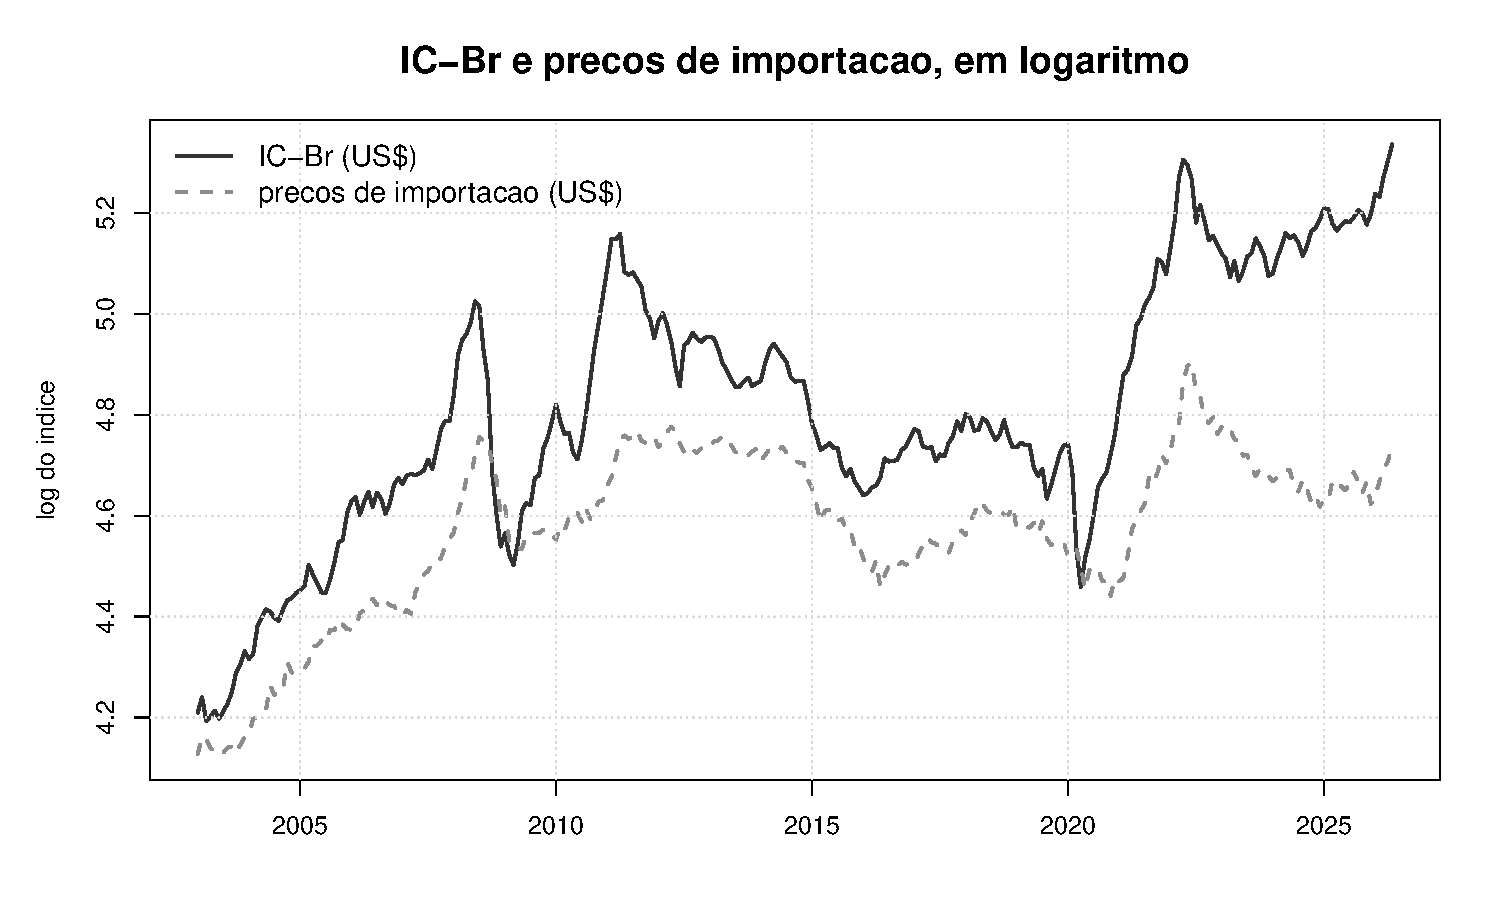
\includegraphics[width=0.85\textwidth]{10_icbr_pimp.pdf}

\vspace{2pt}
\begin{flushleft}\footnotesize
\textit{Nota}: ambos os índices em dólares, em logaritmo do nível. Correlação
de $0{,}87$ entre os níveis e de $0{,}25$ entre as variações mensais. Fonte:
elaboração própria a partir de BCB/SGS e Funcex.
\end{flushleft}
\end{figure}

\subsubsection{Aversão a risco global}

A inclusão de uma variável de risco responde ao argumento de
\citeonline{forbes2018}: o repasse cambial depende da natureza do choque que
move o câmbio. Sem uma variável de risco, movimentos cambiais causados por
aversão a risco global e movimentos causados por melhora dos termos de troca
ficariam indistinguíveis, e o coeficiente estimado de repasse seria apenas uma
média entre os dois. Usa-se o VIX, índice de volatilidade implícita das opções
sobre o S\&P~500, como medida de aversão a risco global. A variável entra em
logaritmo, transformação que reduz a assimetria da série.

\subsubsection{Hiato do produto}

O hiato é construído a partir do IBC-Br dessazonalizado, tomado como
\textit{proxy} mensal da atividade. A tendência é extraída pelo filtro de
Hodrick-Prescott \cite{hodrick1997}, com parâmetro de suavização
$\lambda = 14400$, valor usual para dados mensais, e o hiato é o componente
cíclico resultante, medido em pontos percentuais.

\subsubsection{Taxa de juros}

Usa-se a Selic acumulada no mês e anualizada. A variável de política entra
pela razão dada na Seção~\ref{sec:implicacoes}: a reação do Banco Central faz
parte do mecanismo pelo qual um choque externo chega aos preços, e um sistema
sem ela não mostraria esse caminho. Como efeito secundário, sua presença ajuda
a separar os choques.

\subsubsection{Uma variável deixada de fora}

As expectativas de inflação do Boletim Focus, cujo papel foi discutido na
Seção~\ref{sec:expectativas}, não integram o sistema. A razão é prática: cada
variável adicional consome graus de liberdade de forma significativa, e sete
variáveis já representam um sistema grande para esta amostra.

\subsection{Tratamento das séries}

O IBC-Br é divulgado pelo Banco Central já em versão dessazonalizada. O IPCA é
ajustado sazonalmente pelo procedimento X-13ARIMA-SEATS. As demais séries não
apresentam padrão sazonal relevante e entram sem ajuste.

Todas as observações do período pandêmico foram mantidas, sem exclusões e sem
variáveis binárias. O choque de 2021 e 2022 está no centro do período que se
quer medir, e retirá-lo esvaziaria o exercício. O custo dessa escolha é a
presença de valores extremos capazes de influenciar as estimativas, atenuado
pelos exercícios de subamostra da Seção~\ref{sec:estabilidade}.

% =====================================================================
\section{Análise preliminar: testes de raiz unitária}
\label{sec:estacionariedade}

Antes de estimar o modelo é preciso verificar a ordem de integração das séries.
Estimar um VAR com variáveis não estacionárias produz o risco de regressão
espúria, isto é, de encontrar relações estatisticamente significativas entre
séries que apenas compartilham tendências.

Emprega-se o teste ADF (\textit{Augmented Dickey-Fuller}), cuja hipótese nula é
a presença de raiz unitária. O teste é aplicado com constante e tendência
determinística nas séries em nível, e apenas com constante nas séries em
primeira diferença. Em ambos os casos admite-se até doze defasagens, com a
ordem efetiva escolhida pelo critério de Schwarz. A regra de decisão é direta:
a série entra no sistema na transformação para a qual o ADF rejeita a hipótese
de raiz unitária. Os resultados constam da Tabela~\ref{tab:raizunitaria}.

\begin{table}[htbp]
\centering
\caption{Testes de raiz unitária (ADF)}
\label{tab:raizunitaria}
\footnotesize
\begin{tabular}{lccc}
\toprule
Série & Estatística ADF & Valor crítico (5\%) & Conclusão \\
\midrule
\multicolumn{4}{l}{\textit{Em nível, com constante e tendência}} \\
$\ln p^{c}_t$ \ (IC-Br)             & $-2{,}63$  & $-3{,}42$ & I(1) \\
$\ln p^{m}_t$ \ (preços de import.) & $-2{,}79$  & $-3{,}42$ & I(1) \\
$\ln e_t$ \ (câmbio)                & $-2{,}57$  & $-3{,}42$ & I(1) \\
$i_t$ \ (Selic)\textsuperscript{a}   & $-2{,}49$  & $-2{,}87$ & I(1) \\
\midrule
\multicolumn{4}{l}{\textit{Transformadas, com constante}} \\
$\Delta\ln p^{c}_t$                 & $-8{,}34$  & $-2{,}87$ & I(0) \\
$\Delta\ln p^{m}_t$                 & $-8{,}39$  & $-2{,}87$ & I(0) \\
$\Delta\ln e_t$                     & $-10{,}00$ & $-2{,}87$ & I(0) \\
$\Delta i_t$                        & $-4{,}27$  & $-2{,}87$ & I(0) \\
$v_t$ \ ($\ln$ VIX)                 & $-4{,}55$  & $-2{,}87$ & I(0) \\
$h_t$ \ (hiato)                     & $-6{,}42$  & $-2{,}87$ & I(0) \\
$\pi_t$ \ (IPCA dessazonalizado)    & $-7{,}01$  & $-2{,}87$ & I(0) \\
\bottomrule
\end{tabular}

\vspace{2pt}
\begin{flushleft}\footnotesize
\textit{Nota}: amostra 2003:01--2026:05. H$_0$ do teste ADF: a série tem raiz
unitária. \textsuperscript{a}A Selic é testada apenas com constante, por não
apresentar tendência determinística. Demais séries em nível testadas com
constante e tendência; séries
transformadas, apenas com constante. Número de defasagens escolhido pelo
critério de Schwarz, com máximo de doze. A Selic é testada em nível na primeira
parte da tabela e em primeira diferença na segunda. Fonte: elaboração própria.
\end{flushleft}
\end{table}

As três séries de preços em log-nível, assim como a Selic, não permitem
rejeitar a hipótese de raiz unitária, e portanto são
tratadas como I(1). Suas primeiras diferenças rejeitam a hipótese com folga, o
que confirma que uma diferenciação basta para torná-las estacionárias. O
logaritmo do VIX, o hiato do produto e o IPCA dessazonalizado são estacionários
em nível.

A Selic merece um comentário. Testes de raiz unitária em taxas de juros
costumam ser inconclusivos, porque a série tem persistência muito alta sem ser,
necessariamente, um passeio aleatório. Aqui, o teste não rejeita a raiz
unitária em nenhuma das especificações consideradas, e por isso a variável
entra em primeira diferença. Essa escolha tem a vantagem adicional de deixar o
sistema integralmente estacionário, o que dispensa a discussão de cointegração
e mantém direta a interpretação das funções de resposta a impulso.

% =====================================================================
\section{O modelo VAR}
\label{sec:var}

\subsection{Forma reduzida e escolha das defasagens}

Seja $\mathbf{z}_t$ o vetor de variáveis endógenas do sistema. O modelo
estrutural que descreve a interação entre elas pode ser escrito como

\begin{equation}
\mathbf{B}\mathbf{z}_t = \mathbf{A}_0 + \mathbf{A}_1\mathbf{z}_{t-1}
+ \cdots + \mathbf{A}_p\mathbf{z}_{t-p} + \mathbf{u}_t,
\label{eq:estrutural}
\end{equation}

\noindent em que $\mathbf{B}$ recolhe os efeitos simultâneos entre as
variáveis, as matrizes $\mathbf{A}_j$ recolhem os efeitos defasados e
$\mathbf{u}_t$ é o vetor de choques estruturais, com matriz de covariância
diagonal. Supondo que $\mathbf{B}$ seja inversível, a forma reduzida do sistema
é

\begin{equation}
\mathbf{z}_t = \mathbf{C}_0 + \mathbf{C}_1\mathbf{z}_{t-1}
+ \cdots + \mathbf{C}_p\mathbf{z}_{t-p} + \mathbf{v}_t,
\qquad \mathbf{v}_t = \mathbf{B}^{-1}\mathbf{u}_t,
\label{eq:reduzida}
\end{equation}

\noindent com $\mathbf{C}_j = \mathbf{B}^{-1}\mathbf{A}_j$. É a forma reduzida
que se estima, equação por equação, por mínimos quadrados ordinários. Seus
resíduos $\mathbf{v}_t$ são combinações lineares dos choques estruturais, e por
isso sua matriz de covariância não é diagonal.

O vetor de variáveis é

\begin{equation}
\mathbf{z}_t = \big[\; \underbrace{\Delta\ln p^{c}_t,\ \Delta\ln p^{m}_t,\ v_t}_{\text{bloco externo}},\
\underbrace{h_t,\ \pi_t,\ \Delta i_t,\ \Delta\ln e_t}_{\text{bloco doméstico}} \;\big]'.
\label{eq:vetor}
\end{equation}

A ordem de defasagens é escolhida comparando os critérios de informação de
Akaike, Hannan-Quinn e Schwarz, com máximo de doze meses. Os três critérios
apontam ordens baixas, entre uma e duas defasagens. Especificações tão curtas,
porém, deixam autocorrelação nos resíduos, o que violaria uma hipótese básica
do modelo. Adota-se, por isso, a regra de escolher a menor ordem que elimine a
autocorrelação residual, verificada pelo teste de Breusch-Godfrey. Sob esse
critério, a ordem selecionada é $p = 5$. Em todas as especificações mais curtas
a equação da Selic apresenta autocorrelação residual significativa.

O modelo é submetido a duas verificações. A estabilidade é avaliada pelo módulo
das raízes do polinômio característico, que devem ser menores que a unidade. A
estabilidade estrutural dos coeficientes é avaliada pelo teste CUSUM aplicado
aos resíduos recursivos de cada equação. Os intervalos de confiança das funções
de resposta são construídos por \textit{bootstrap}, com mil replicações nas
respostas do sistema completo e quinhentas nos exercícios que exigem reestimação
do modelo em cada replicação.

\subsection{Identificação}

A forma reduzida não permite interpretação econômica direta. Um resíduo grande
na equação do câmbio pode ser um choque cambial de verdade, mas pode ser também
a reação do câmbio a um choque de commodities ocorrido no mesmo mês. Separar as
duas coisas exige recuperar $\mathbf{B}$. Esse é o problema da identificação: a
forma estrutural tem mais parâmetros que a forma reduzida, e por isso o sistema
que liga uma à outra admite infinitas soluções.

A solução adotada é a decomposição de Cholesky, que dá a $\mathbf{B}$ uma forma
triangular. Na prática, isso é ordenar as variáveis da mais lenta para a mais
rápida: dentro do mesmo mês, cada variável só pode ser afetada pelas que vêm
antes dela na fila. A ordem usada é a da equação~\eqref{eq:vetor}, e cada
posição tem uma justificativa.

O bloco externo vem antes do doméstico porque o Brasil é uma economia pequena e
aberta. Preços internacionais de commodities, preços de importação e o clima de
risco global são determinados lá fora, em mercados nos quais o país é tomador de
preços.

Dentro do bloco externo, as commodities vêm antes dos preços de importação,
porque produtos primários são insumo dos manufaturados que o Brasil compra. O
VIX fica por último no bloco, por ser uma variável financeira e reagir mais
rápido que as outras duas.

No bloco doméstico, atividade e inflação vêm primeiro. A hipótese é a
convencional: decisões de produção e preços já contratados não mudam dentro do
mês por causa de novidades financeiras. Depois vem a Selic, porque o Banco
Central olha atividade e inflação antes de decidir. E o câmbio fica em último
lugar, por ser a variável que se ajusta mais depressa.

Com o câmbio em último lugar, o choque associado a ele é, por construção,
independente de todos os demais. Ele representa um choque cambial puro, e não
um movimento cambial qualquer, que é justamente o que interessa medir, pelo
argumento de \citeonline{forbes2018}.

Ainda assim, a ordem adotada é necessariamente arbitrária. Outras hipóteses
igualmente defensáveis levariam a outras ordens, e os resultados são
condicionais à escolha feita. Por isso o
Capítulo~\ref{cap:resultados} traz um exercício que reestima o modelo sob
ordenações alternativas.

% =====================================================================
\section{Ferramentas de análise}
\label{sec:ferramentas}

\subsection{Funções de resposta a impulso}
\label{sec:fri}

A função de resposta a impulso descreve a trajetória de cada variável do
sistema após um choque estrutural. É o instrumento central do trabalho. As
respostas são reportadas para um horizonte de 24 meses, com intervalos de
confiança de 90\% obtidos por \textit{bootstrap}.

O objeto de interesse é a resposta \textit{acumulada} do IPCA. Como o IPCA
entra no sistema em variação mensal, a soma de suas respostas até o horizonte
$n$ equivale à resposta do nível de preços nesse horizonte.

Resta definir por quanto essa resposta é dividida. O choque estimado pelo
modelo tem o tamanho de um desvio padrão, o que não permite leitura econômica
direta.
A tentação é dividir pelo movimento da variável de origem no mês do impacto,
mas isso seria errado: a variável não para no primeiro mês, ela continua
respondendo ao próprio choque durante algum tempo, e é a variação acumulada
dela que importa para a variação acumulada do nível de preços. O repasse é,
portanto,

\begin{equation}
\beta_{n} \;=\;
\frac{\text{resposta acumulada do IPCA}}
     {\text{variação acumulada da variável de origem}} ,
\label{eq:repasse}
\end{equation}

\noindent com numerador e denominador medidos no mesmo horizonte $n$. É a
versão empírica do coeficiente definido em~\eqref{eq:erpt}: o numerador é a
resposta acumulada do IPCA ao choque, e o denominador é a resposta acumulada da
própria variável de origem ao mesmo choque. Lido assim, o número responde à
pergunta: quanto o nível de preços subiu para cada 1\% de variação acumulada
da variável de interesse?

Como o repasse é uma razão entre duas respostas estimadas, o intervalo de
confiança precisa vir de um \textit{bootstrap} da própria razão. Usar as
bandas do numerador ignoraria a incerteza do denominador.

\subsection{O papel do câmbio}
\label{sec:papelcambio}

O câmbio cumpre papel duplo diante de um choque de commodities. Ele transmite
parte do choque aos preços, mas também o amortece, porque a alta das cotações
internacionais tende a apreciar o real.

O problema de medir esse amortecimento é que a resposta do IPCA estimada pelo
VAR já é um efeito total, com o câmbio se movendo dentro dela. Não existe, nos
dados, um mundo em que o mesmo choque ocorra sem que o câmbio reaja. Esse mundo
precisa ser construído.

O procedimento adotado é o de \citeonline{simszha2006}, tal como aplicado por
\citeonline{bernanke1997} ao papel da política monetária na transmissão de
choques de petróleo. A resposta da inflação ao choque de commodities é estimada
duas vezes. Na primeira, o câmbio responde livremente, e o resultado é a função
de resposta a impulso usual. Na segunda, o câmbio é mantido na trajetória que
teria sem o choque. Para isso, a cada mês do horizonte injeta-se no sistema uma
inovação cambial do tamanho exato do movimento que o câmbio faria, com sinal
contrário. Como a dinâmica do modelo volta a deslocá-lo no mês seguinte, a
compensação precisa ser refeita período a período. A contribuição do canal
cambial é a diferença entre as duas trajetórias:

\begin{equation}
\mathrm{Canal}_{n} \;=\; R_{n} \;-\; R^{\,\mathrm{cf}}_{n} ,
\label{eq:canalcambio}
\end{equation}

\noindent em que $R_{n}$ é a resposta acumulada do IPCA ao choque de
commodities no horizonte $n$, com o câmbio livre, e $R^{\,\mathrm{cf}}_{n}$ é
a mesma resposta com o câmbio neutralizado. Como a alta das commodities aprecia o real,
espera-se que a resposta contrafactual seja maior que a observada e que
$\mathrm{Canal}_{n}$ seja negativo, indicando que o câmbio segurou parte da
inflação que o choque teria gerado.

Três decisões de implementação precisam ficar registradas.

Manter o câmbio parado quer dizer mantê-lo na trajetória que ele teria sem o
choque, e não em um nível fixo.

O câmbio é segurado desde o próprio mês do choque. Isso poderia ser um
problema, porque o choque compensatório também mexe na inflação, mas na
ordenação de Cholesky adotada o câmbio vem depois do IPCA, e uma inovação
cambial não afeta a inflação dentro do mesmo mês. Segurar o câmbio só a partir
do mês seguinte produz resultados próximos.

Os intervalos de confiança vêm de um \textit{bootstrap} em que cada replicação
reestima o VAR e refaz o contrafactual do zero, em vez de reamostrar mantendo
os coeficientes fixos.

Convém dizer também o que a medida não é. A diferença em~\eqref{eq:canalcambio}
captura todos os caminhos que passam pelo câmbio, inclusive os indiretos, como o que vai
das commodities ao câmbio, deste à Selic e daí à inflação. Ela não isola o
caminho direto do câmbio para os preços, e depende da identificação adotada. Por
isso o resultado é reportado em pontos percentuais, e não como proporção do
efeito total: como a resposta estimada é pequena, essa razão seria instável.

\subsection{Decomposição da variância e causalidade}

Dois instrumentos complementam a leitura das funções de resposta.

A decomposição da variância do erro de previsão mede a fração da variabilidade
não antecipada do IPCA atribuível a cada choque estrutural, nos horizontes de
3, 12 e 24 meses. É esse instrumento que responde, em média para toda a
amostra, à pergunta sobre o peso relativo dos três vetores externos formulada
no Capítulo~\ref{cap:introducao}.

O teste de causalidade de Granger verifica se o conhecimento dos valores
passados de uma variável ajuda a prever as demais. Aplicado aos choques
externos, ele oferece uma verificação preliminar e simples de que essas
variáveis de fato carregam informação sobre a inflação doméstica.

% =====================================================================
\section{O repasse é estável?}
\label{sec:estabilidade}

A Seção~\ref{sec:naolinear-lit} documentou que o repasse cambial não é
necessariamente constante. Esta seção descreve dois exercícios simples que
verificam se essas variações aparecem nos dados brasileiros.

\subsection{O repasse mudou ao longo do tempo?}

Supor coeficientes constantes ao longo de 280 meses que cobrem o \textit{boom}
de commodities, a crise financeira global, a recessão de 2015 e 2016 e a
pandemia é pouco plausível. Para avaliar isso, o modelo é
reestimado em duas janelas, 2003:02 a 2013:12 e 2014:01 a 2026:05, e as
respostas acumuladas do IPCA ao choque cambial em doze meses são comparadas.

A divisão em 2014 não é arbitrária: marca aproximadamente o fim do ciclo de
alta das commodities e o início do período de deterioração fiscal e cambial. O
exercício permite verificar se o declínio do repasse documentado por
\citeonline{nogueirajr2007} para o período de consolidação do regime de metas
se mantém no período recente. Como cada subamostra tem cerca de 140 observações, a precisão das estimativas
é menor, e por isso os intervalos de confiança das duas janelas são comparados
explicitamente.

Convém deixar claro o alcance do exercício. Comparar dois intervalos de
confiança não é um teste formal de igualdade entre os coeficientes. O que se
obtém é evidência indicativa sobre a direção da mudança, e não um resultado
com nível de significância associado.

\subsection{Depreciações e apreciações têm o mesmo efeito?}

A literatura sugere que depreciações são repassadas com mais intensidade que
apreciações de mesma magnitude, padrão consistente com a rigidez de preços à
queda. Para verificar isso, estima-se uma regressão auxiliar que separa a
variação cambial em suas parcelas positiva e negativa:

\begin{equation}
\pi_t = \alpha
+ \sum_{j=0}^{6}\left( \beta^{+}_j\,\Delta e^{+}_{t-j}
                     + \beta^{-}_j\,\Delta e^{-}_{t-j} \right)
+ \gamma_1 \pi_{t-1} + \gamma_2 \pi_{t-2} + \nu_t .
\label{eq:assimetria}
\end{equation}

A variação cambial do mês foi partida em duas: $\Delta e^{+}_t$ guarda os
meses de depreciação e vale zero nos demais, e $\Delta e^{-}_t$ guarda os
meses de apreciação. Entram também seis defasagens de cada parcela, porque o
repasse não é imediato, e duas defasagens da própria inflação, para controlar
a inércia.

Se o repasse fosse simétrico, a soma dos coeficientes de um lado seria igual à
do outro. É isso que o teste de Wald verifica. Somas diferentes, com a das
depreciações maior, indicariam repasse mais intenso quando o dólar sobe.

Este exercício é ilustrativo e tem alcance menor que o do VAR. Por ser uma
equação única, ele trata a variação cambial como se fosse exógena à inflação,
quando na verdade as duas se determinam em conjunto. É exatamente esse
problema que a identificação do VAR resolve, e que a regressão auxiliar não
resolve. O resultado deve ser lido como um indício, não como estimativa do
repasse.

% =====================================================================
\section{Limitações da estratégia empírica}
\label{sec:limitacoes}

O trabalho tem seis limitações.

Primeiro, o tamanho do sistema. Sete variáveis são o mínimo para acomodar os
canais discutidos no Capítulo~\ref{cap:revisao}, mas já consomem boa parte dos
graus de liberdade. Outros canais relevantes, como separar o IPCA entre preços
livres e administrados, ficariam melhor em sistemas menores.

Segundo, a identificação por Cholesky, embora padrão na literatura, depende da
ordem em que o pesquisador coloca as variáveis. Os resultados valem para a
ordem escolhida.

Terceiro, o contrafactual da Seção~\ref{sec:papelcambio} é uma
intervenção sobre o modelo estimado, e não a descrição de um regime cambial
alternativo. Ele mede o que desaparece da resposta da inflação quando o câmbio
é impedido de se mover, o que inclui todos os caminhos que passam por ele, e
depende da identificação adotada.

Quarto, manter o período pandêmico é necessário para o objetivo do trabalho,
mas traz observações de magnitude excepcional. A influência delas sobre as
estimativas pode ser atenuada, não eliminada. Os exercícios de subamostra da
Seção~\ref{sec:estabilidade} ajudam, mas não resolvem.

Quinto, o IC-Br é construído com pesos que já refletem a importância de cada
commodity para a inflação brasileira, como registrado na
Seção~\ref{sec:variaveis}. Parte da relação estimada com o IPCA pode, por
isso, ser mecânica. Uma verificação com índice internacional cujos pesos não
dependam da inflação doméstica seria o passo natural, e fica como extensão.

Sexto, a ordenação de Cholesky impede que choques domésticos afetem as
variáveis externas no mesmo mês, mas ainda permite que as defasagens das
domésticas apareçam nas equações das externas. Um VAR com exogeneidade em
bloco zeraria também esses coeficientes e seria mais adequado à hipótese de
economia pequena e aberta. A estimação desse modelo foge ao escopo deste
trabalho.

Nenhuma dessas limitações compromete o objetivo central, que é medir a
contribuição relativa dos três vetores externos e o papel do câmbio no período
recente, mas todas condicionam a leitura dos resultados apresentados no
Capítulo~\ref{cap:resultados}.


%=======================================================================
% CAPÍTULO 4
%=======================================================================
\chapter{Resultados}
\label{cap:resultados}

Este capítulo apresenta os resultados do modelo descrito no
Capítulo~\ref{cap:dados}. A ordem segue a das perguntas formuladas na introdução. Primeiro vêm os
diagnósticos do modelo. Depois, o efeito de cada choque externo sobre a
inflação. Em seguida, o papel do câmbio nessa transmissão e o peso relativo
dos choques. As três últimas seções verificam se o repasse é estável, se os
resultados dependem da ordenação escolhida e como eles se comparam à
literatura.

% ---------------------------------------------------------------------
\section{Diagnósticos do modelo}
\label{sec:diagnosticos}

O sistema foi estimado com cinco defasagens, pela regra descrita na
Seção~\ref{sec:var}. Três verificações precedem a leitura dos
resultados.

Sobre estabilidade, todas as raízes do polinômio característico têm módulo
inferior à unidade, e a maior delas fica em torno de $0{,}93$. O sistema é
estável, ainda que com persistência alta, o que era de se esperar em um modelo
mensal com variáveis financeiras.

Sobre autocorrelação residual, o teste de Breusch-Godfrey não rejeita a
hipótese de resíduos não correlacionados a 5\%, tanto com uma quanto com duas
defasagens. Em todas as especificações mais curtas o teste rejeitava, e foi
isso que levou à escolha de $p = 5$.

Sobre a estabilidade dos coeficientes ao longo do tempo, o teste CUSUM,
aplicado equação por equação, mantém as estatísticas dentro das bandas em
todas elas. Os gráficos são gerados pelo segundo script e estão disponíveis no repositório
indicado na Seção~\ref{sec:reprodutibilidade}.

% ---------------------------------------------------------------------
\section{Os choques externos e a inflação}
\label{sec:resultadosfri}

As Figuras~\ref{fig:pontuais} e~\ref{fig:acumuladas} mostram a resposta do
IPCA aos três choques externos, primeiro mês a mês e depois acumulada. A
Tabela~\ref{tab:fri} resume a versão acumulada em três horizontes, já na forma
de coeficiente de repasse definida em~\eqref{eq:repasse}.

\begin{table}[htbp]
\centering
\caption{Repasse acumulado ao IPCA}
\label{tab:fri}
\footnotesize
\begin{tabular}{lcccc}
\toprule
Choque & Horizonte & Repasse (\%) & \multicolumn{2}{c}{Intervalo de 90\%} \\
\cmidrule(lr){4-5}
       & (meses)   &               & Inferior & Superior \\
\midrule
\multirow{3}{*}{Commodities}
  & 6  & $0{,}049$ & $0{,}022$ & $0{,}081$ \\
  & 12 & $0{,}059$ & $0{,}015$ & $0{,}118$ \\
  & 24 & $0{,}061$ & $0{,}010$ & $0{,}124$ \\
\midrule
\multirow{3}{*}{Preços de importação}
  & 6  & $-0{,}021$ & $-0{,}111$ & $0{,}049$ \\
  & 12 & $-0{,}023$ & $-0{,}163$ & $0{,}075$ \\
  & 24 & $-0{,}013$ & $-0{,}160$ & $0{,}107$ \\
\midrule
\multirow{3}{*}{Câmbio}
  & 6  & $0{,}051$ & $0{,}024$ & $0{,}087$ \\
  & 12 & $0{,}079$ & $0{,}039$ & $0{,}132$ \\
  & 24 & $0{,}100$ & $0{,}046$ & $0{,}185$ \\
\bottomrule
\end{tabular}

\vspace{2pt}
\begin{flushleft}\footnotesize
\textit{Nota}: resposta acumulada do IPCA dividida pela variação acumulada da
variável de origem no mesmo horizonte, conforme a equação~\eqref{eq:repasse}.
Lê-se como a variação percentual do nível de preços por cada 1\% de variação
acumulada da variável de origem. Identificação por Cholesky na ordenação da
equação~\eqref{eq:vetor}. Intervalos de 90\% por \textit{bootstrap} da razão,
com mil replicações e reestimação do modelo em cada uma. Fonte: elaboração
própria.
\end{flushleft}
\end{table}

\begin{figure}[htbp]
\centering
\caption{Resposta mensal do IPCA aos choques externos}
\label{fig:pontuais}
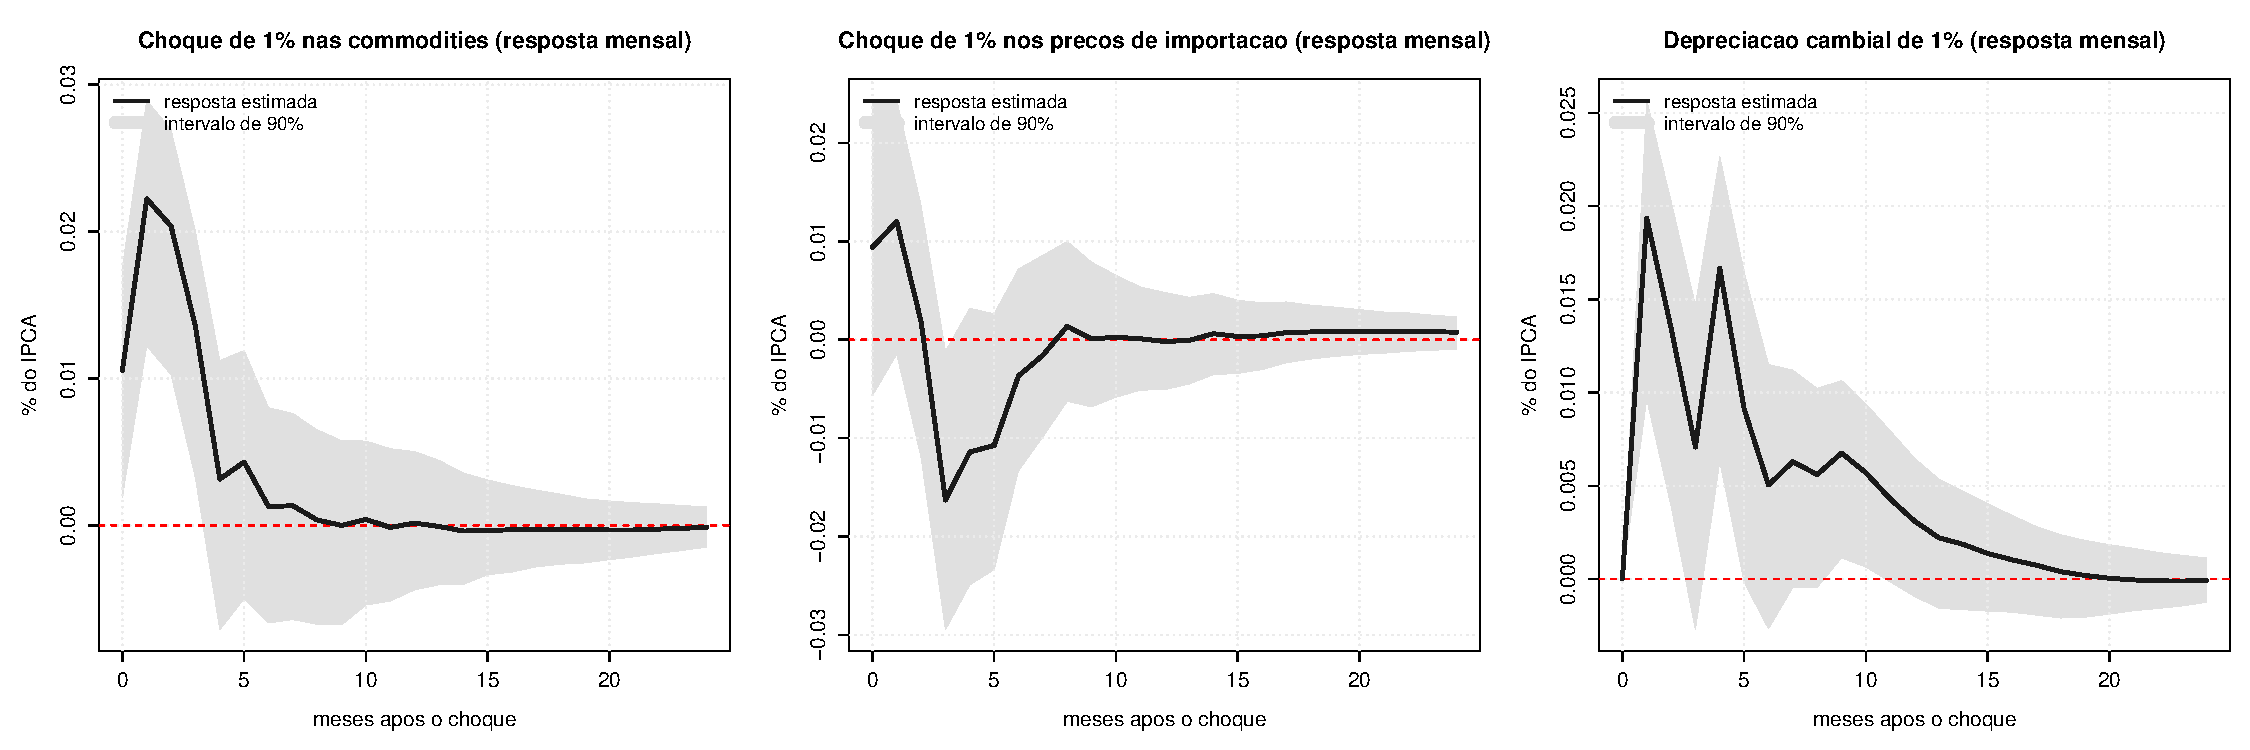
\includegraphics[width=\textwidth]{08_respostas_pontuais.pdf}

\vspace{2pt}
\begin{flushleft}\footnotesize
\textit{Nota}: resposta do IPCA em cada mês após o choque, não acumulada.
Bandas de 90\% por \textit{bootstrap}. Fonte: elaboração própria.
\end{flushleft}
\end{figure}

\begin{figure}[htbp]
\centering
\caption{Resposta acumulada do IPCA aos choques externos}
\label{fig:acumuladas}
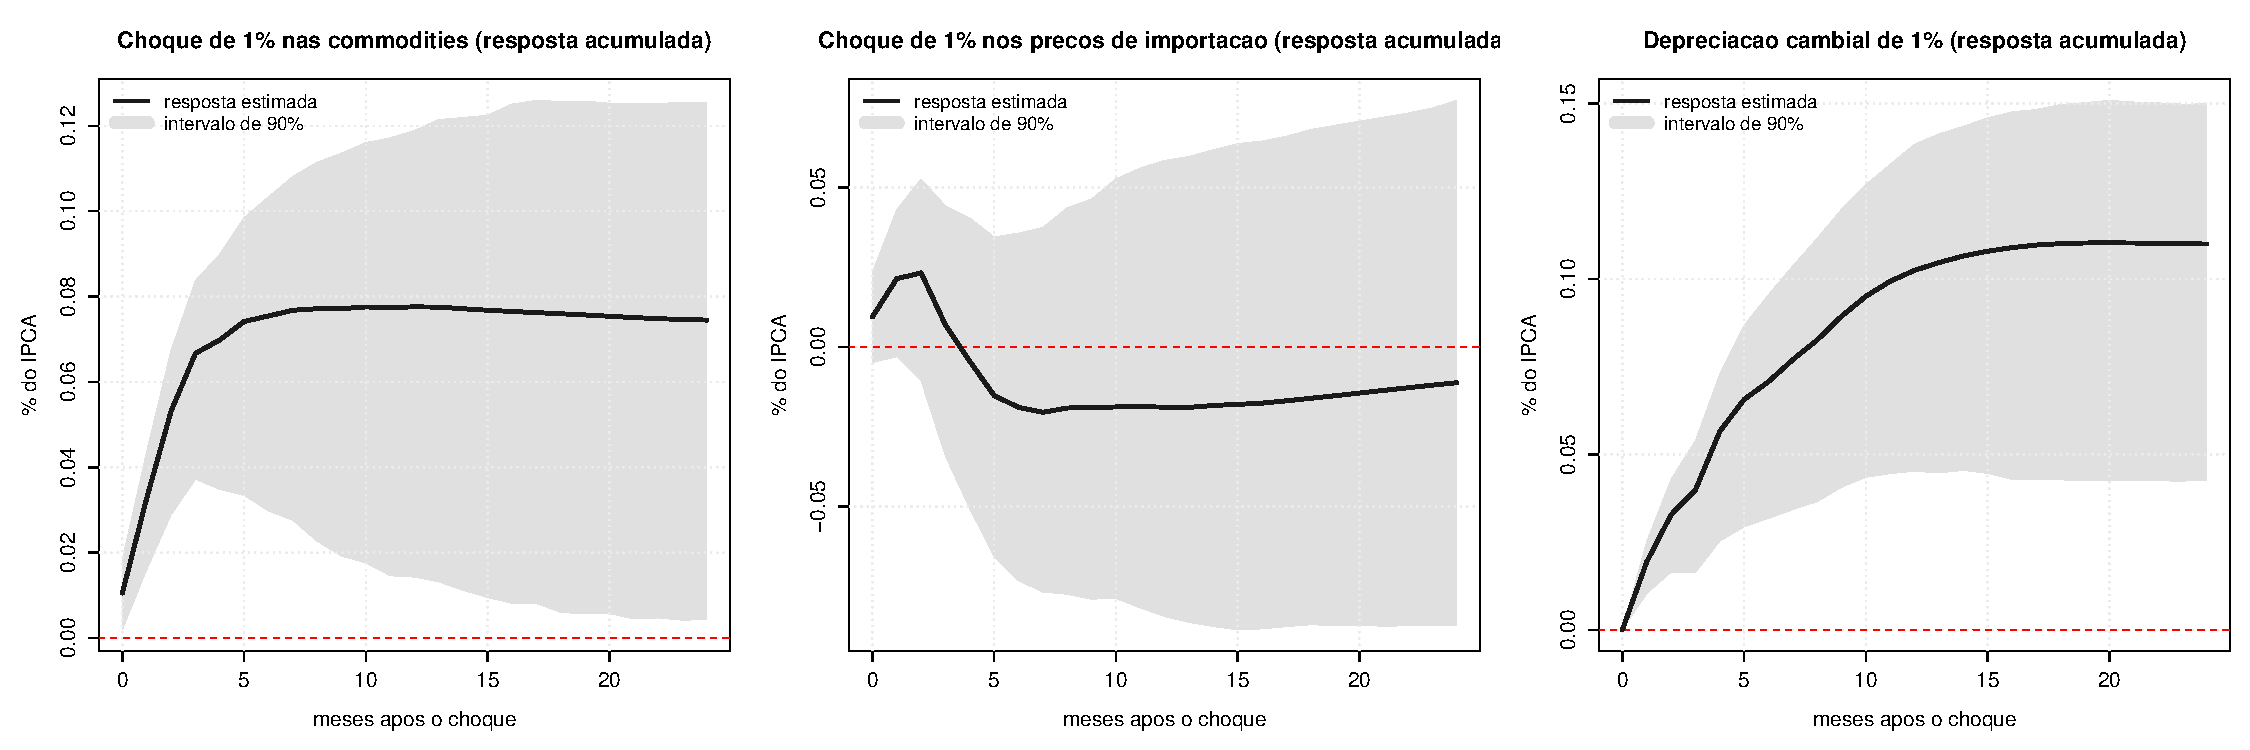
\includegraphics[width=\textwidth]{09_respostas_acumuladas.pdf}

\vspace{2pt}
\begin{flushleft}\footnotesize
\textit{Nota}: soma das respostas mensais até cada horizonte, que equivale ao
efeito sobre o nível de preços. Bandas de 90\% por \textit{bootstrap}. Fonte:
elaboração própria.
\end{flushleft}
\end{figure}

A leitura das duas figuras é direta. O efeito mensal aparece nos primeiros
meses e depois se dissipa, o que faz a curva acumulada subir no início e
estabilizar. A resposta ao choque cambial é a que demora mais a se completar.

Três pontos chamam atenção.

O choque de commodities eleva o nível de preços em $0{,}059\%$ ao fim de doze
meses, com intervalo de confiança que exclui o zero. O repasse cresce com o
horizonte, de $0{,}049\%$ aos seis meses para $0{,}061\%$ aos vinte e quatro,
mas a maior parte já se realizou no primeiro ano. Isso é coerente com a
natureza do choque, que chega aos preços domésticos sobretudo por alimentos e
combustíveis, itens de repasse rápido.

O choque cambial produz o maior efeito dos três, $0{,}079\%$ em doze meses, e
segue crescendo até $0{,}100\%$ no vigésimo quarto. A comparação com o
resultado anterior é informativa: o câmbio transmite mais e transmite por mais
tempo que as commodities. O repasse é claramente incompleto, bem abaixo da
unidade, o que é coerente com o quadro descrito na Seção~\ref{sec:metas}, em
que a consolidação do regime de metas reduziu a transmissão de choques
cambiais aos preços.

O choque de preços de importação não produz efeito estatisticamente distinto de
zero em nenhum dos horizontes. O ponto estimado é inclusive negativo, ainda que
próximo de zero. Esse resultado não deve ser lido como ausência de inflação
importada: ele indica que, uma vez controlados o preço internacional das
commodities e o câmbio, o índice de preços de importação não acrescenta
informação sobre a inflação brasileira. Ou seja, os dois primeiros canais parecem captar o que há para captar.

% ---------------------------------------------------------------------
\section{O papel do câmbio na transmissão}
\label{sec:resultadocanal}

A Seção~\ref{sec:papelcambio} descreveu o exercício contrafactual, que segue o
procedimento de \citeonline{simszha2006} aplicado por
\citeonline{bernanke1997}. A Tabela~\ref{tab:canalcambio} traz o resultado e a
Figura~\ref{fig:contrafactual} mostra as duas trajetórias.

\begin{table}[htbp]
\centering
\caption{Decomposição da resposta do IPCA ao choque de commodities}
\label{tab:canalcambio}
\footnotesize
\begin{tabular}{lccc}
\toprule
Horizonte (meses) & 6 & 12 & 24 \\
\midrule
Repasse observado (\%)            & $0{,}049$ & $0{,}059$ & $0{,}061$ \\
Repasse sem o canal cambial (\%)  & $0{,}081$ & $0{,}101$ & $0{,}104$ \\
Contribuição do câmbio (p.p.)     & $-0{,}032$ & $-0{,}042$ & $-0{,}043$ \\
\quad Intervalo de 90\%           & $[-0{,}057;\,-0{,}016]$
                                  & $[-0{,}082;\,-0{,}014]$
                                  & $[-0{,}088;\,-0{,}010]$ \\
\bottomrule
\end{tabular}

\vspace{2pt}
\begin{flushleft}\footnotesize
\textit{Nota}: a resposta sem o canal cambial é obtida mantendo o câmbio na
trajetória que teria sem o choque, por meio de inovações compensatórias
período a período, conforme a equação~\eqref{eq:canalcambio}. A contribuição do
câmbio é a diferença entre as duas linhas anteriores. Valores negativos indicam
que o câmbio reduziu a inflação que o choque teria gerado. Intervalos de 90\%
por \textit{bootstrap} com quinhentas replicações, com reestimação do modelo em
cada replicação. Fonte: elaboração própria.
\end{flushleft}
\end{table}

\begin{figure}[htbp]
\centering
\caption{Resposta do IPCA a um choque de 1\% nas commodities}
\label{fig:contrafactual}
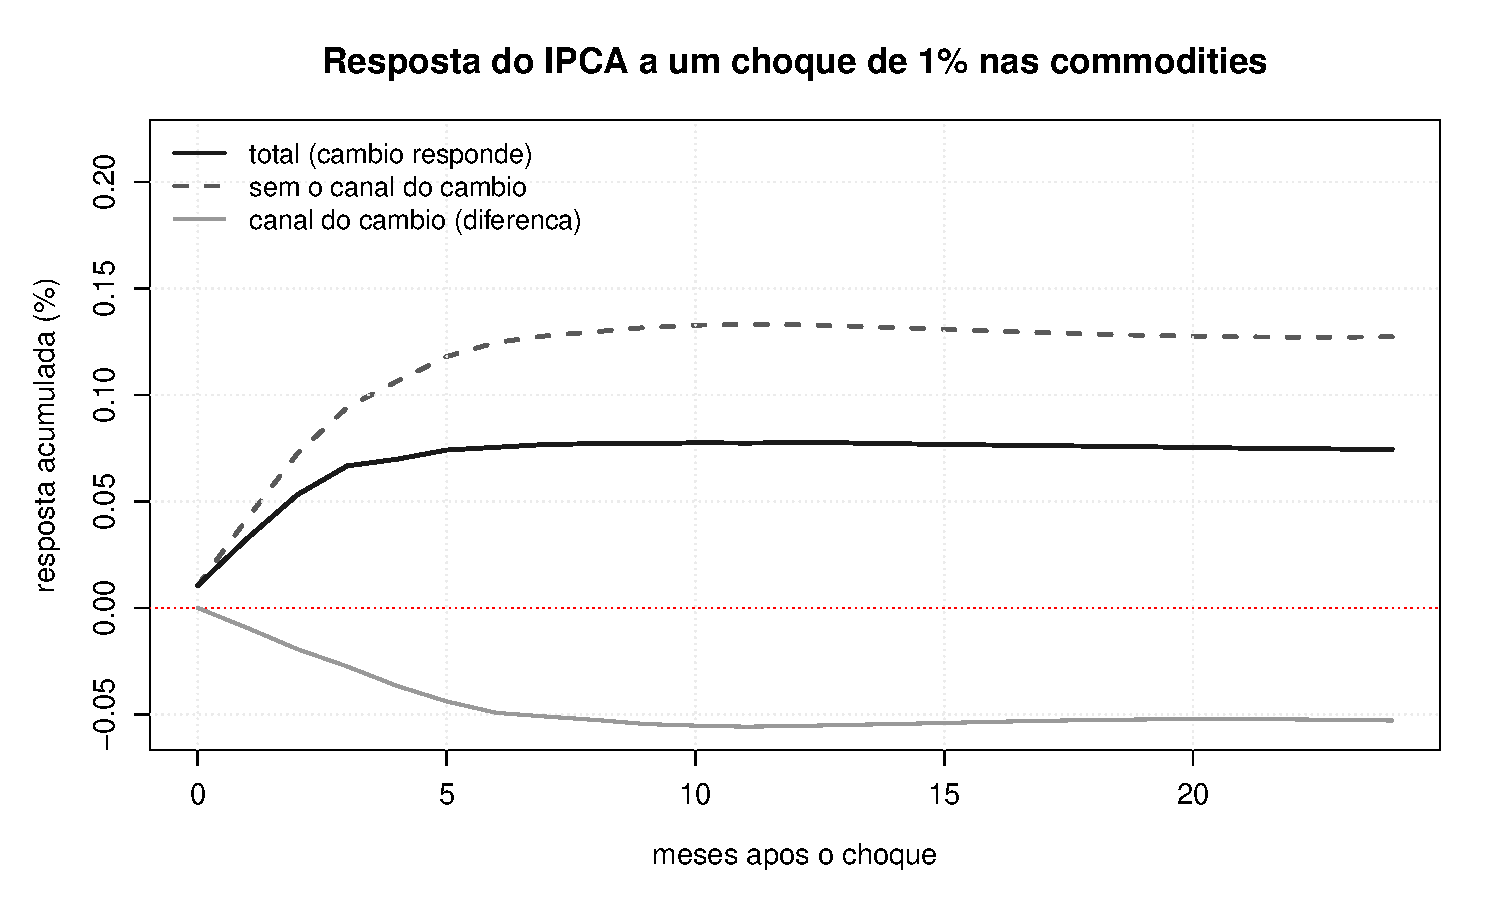
\includegraphics[width=0.85\textwidth]{07_contrafactual.pdf}

\vspace{2pt}
\begin{flushleft}\footnotesize
\textit{Nota}: respostas acumuladas. A linha cheia é a resposta estimada pelo
modelo. A linha tracejada é a resposta contrafactual, com o câmbio mantido
parado. A linha inferior é a diferença entre as duas. Fonte: elaboração
própria.
\end{flushleft}
\end{figure}

O resultado vai na direção esperada. Se o câmbio não pudesse reagir, o mesmo
choque de commodities teria elevado o nível de preços em $0{,}101\%$ ao fim de
doze meses, contra os $0{,}059\%$ efetivamente estimados. A diferença,
$0{,}042$ ponto percentual, é a parcela do choque absorvida pela apreciação do
real, e o intervalo de confiança exclui o zero nos três horizontes.

A leitura econômica é a de que o câmbio funciona como amortecedor. A alta das
cotações internacionais melhora os termos de troca brasileiros, aprecia o real
e barateia o componente importado da cesta de consumo, o que compensa parte do
encarecimento direto dos alimentos e combustíveis. O trabalho de
\citeonline{stockl2017} descreve esse mecanismo para economias exportadoras de
commodities, e os dados brasileiros o reproduzem.

O número exige duas ressalvas. Os $0{,}042$ ponto percentual não medem só o
caminho que vai do câmbio para os preços: medem tudo que desaparece quando o
câmbio para de se mover, incluindo a reação da Selic à apreciação e o efeito
dessa reação sobre a inflação. E o exercício supõe que os coeficientes
estimados continuariam valendo num cenário de câmbio imóvel, de modo que ele
não descreve o que aconteceria sob outro regime cambial.

O procedimento foi verificado de duas formas. Na trajetória contrafactual, a
resposta acumulada do câmbio é nula em todos os horizontes, até a precisão
numérica do cálculo, o que confirma que as inovações compensatórias de fato o
mantiveram parado. E o exercício foi refeito segurando o câmbio apenas a
partir do primeiro mês, em vez do mês do impacto, com resultados próximos.

Uma última observação sobre a ordem de grandeza. O amortecimento corresponde a algo próximo de dois quintos do efeito que o
choque teria sem a resposta cambial. Como a resposta total é pequena em termos absolutos, essa
proporção é sensível a variações modestas nas estimativas, e por isso o
resultado é reportado em pontos percentuais.

% ---------------------------------------------------------------------
\section{O peso relativo dos choques externos}
\label{sec:resultadofevd}

A decomposição da variância do erro de previsão, na
Tabela~\ref{tab:fevd}, responde à primeira pergunta da introdução: qual dos
vetores externos pesa mais na dinâmica recente do IPCA.

\begin{table}[htbp]
\centering
\caption{Decomposição da variância do erro de previsão do IPCA (\%)}
\label{tab:fevd}
\footnotesize
\begin{tabular}{lccccccc}
\toprule
Horizonte & Commodities & P. import. & VIX & Hiato & IPCA & Selic & Câmbio \\
\midrule
3 meses  & $13{,}0$ & $1{,}0$ & $0{,}7$ & $0{,}4$ & $79{,}0$ & $0{,}1$ & $5{,}8$ \\
12 meses & $12{,}7$ & $2{,}7$ & $3{,}9$ & $0{,}8$ & $66{,}3$ & $3{,}9$ & $9{,}7$ \\
24 meses & $12{,}6$ & $2{,}7$ & $4{,}6$ & $0{,}8$ & $65{,}7$ & $3{,}9$ & $9{,}8$ \\
\bottomrule
\end{tabular}

\vspace{2pt}
\begin{flushleft}\footnotesize
\textit{Nota}: percentual da variância do erro de previsão do IPCA atribuível a
cada choque estrutural. As linhas somam cem por cento, a menos de
arredondamento. Fonte: elaboração própria.
\end{flushleft}
\end{table}

Entre os choques externos, o de commodities é o mais importante, respondendo por
cerca de $12{,}7\%$ da variância do IPCA em doze meses, seguido pelo câmbio, com
$9{,}7\%$. O VIX responde por $3{,}9\%$ e os preços de importação por apenas
$2{,}7\%$, o que reforça a leitura da seção anterior. Somados, os quatro choques
externos explicam cerca de trinta por cento da variabilidade não antecipada da
inflação em doze meses.

Cabe explicar por que essa ordem difere da Tabela~\ref{tab:fri}, em que o
choque cambial produzia o maior efeito. As duas medidas respondem a perguntas
diferentes. A função de resposta a impulso mede o efeito de um choque de tamanho
fixo, 1\% em cada caso, e diz qual canal é mais potente por unidade. A
decomposição da variância pondera cada canal também pela frequência e pela
magnitude com que seus choques de fato ocorreram na amostra. O choque de
commodities é mais volátil que o choque cambial puro, e por isso responde por
mais variância do IPCA mesmo tendo efeito menor por unidade. Os dois resultados
são complementares, e não contraditórios.

A maior parte da variância continua sendo explicada pelo próprio choque de
inflação, $66{,}3\%$ em doze meses. Isso não indica falha do modelo. Reflete a inércia inflacionária e o fato de
que boa parte da variação do IPCA vem de fatores próprios, como preços
administrados e choques setoriais, que o sistema não modela em separado.

Os testes de causalidade de Granger, na Tabela~\ref{tab:granger}, apontam na
mesma direção.

\begin{table}[htbp]
\centering
\caption{Causalidade de Granger}
\label{tab:granger}
\footnotesize
\begin{tabular}{lccc}
\toprule
Variável & Estatística $F$ & Graus de liberdade & Valor-$p$ \\
\midrule
Commodities            & $3{,}36$ & $(30;\,1673)$ & $<0{,}001$ \\
Preços de importação   & $1{,}52$ & $(30;\,1673)$ & $0{,}036$ \\
Câmbio                 & $1{,}82$ & $(30;\,1673)$ & $0{,}005$ \\
\bottomrule
\end{tabular}

\vspace{2pt}
\begin{flushleft}\footnotesize
\textit{Nota}: H$_0$ do teste: a variável indicada não causa, no sentido de
Granger, as demais variáveis do sistema. Fonte: elaboração própria.
\end{flushleft}
\end{table}

As três variáveis externas ajudam a prever as demais, com rejeição da hipótese
nula a 1\% para as commodities e para o câmbio, e a 5\% para os preços de
importação. O teste confirma que as séries carregam informação sobre a dinâmica
doméstica, ainda que não informe o sinal nem a magnitude dos efeitos.

% ---------------------------------------------------------------------
\section{O repasse é estável?}
\label{sec:resultadoestabilidade}

Os dois exercícios descritos na Seção~\ref{sec:estabilidade} verificam se o
repasse cambial se comporta de modo homogêneo ao longo da amostra e entre
depreciações e apreciações.

\subsection{Subamostras}

A Tabela~\ref{tab:subamostras} compara a resposta acumulada do IPCA ao choque
cambial em doze meses nas duas janelas.

\begin{table}[htbp]
\centering
\caption{Repasse cambial em doze meses, por subamostra}
\label{tab:subamostras}
\footnotesize
\begin{tabular}{lcccc}
\toprule
Janela & Observações & Resposta (\%) & \multicolumn{2}{c}{Intervalo de 90\%} \\
\cmidrule(lr){4-5}
       &             &               & Inferior & Superior \\
\midrule
2003:02 a 2013:12 & $131$ & $0{,}022$ & $-0{,}032$ & $0{,}093$ \\
2014:01 a 2026:05 & $149$ & $0{,}113$ & $0{,}042$  & $0{,}238$ \\
\bottomrule
\end{tabular}

\vspace{2pt}
\begin{flushleft}\footnotesize
\textit{Nota}: modelo reestimado em cada janela, com a mesma especificação e a
mesma ordenação. Intervalos de 90\% por \textit{bootstrap} com quinhentas
replicações. Fonte: elaboração própria.
\end{flushleft}
\end{table}

O contraste é grande. Na primeira janela o repasse é de $0{,}022\%$ e o
intervalo de confiança inclui o zero, isto é, não se pode afirmar que houvesse
repasse mensurável. Na segunda ele é de $0{,}113\%$, cerca de cinco vezes
maior, e o intervalo exclui o zero.

A tentação é concluir que o repasse aumentou. A conclusão, porém, exige cautela. Os intervalos se sobrepõem na faixa entre
$0{,}042$ e $0{,}093$, o que é esperado quando cada subamostra tem cerca de
$140$ observações para um sistema de sete variáveis e cinco defasagens. E,
mais importante, comparar dois intervalos não constitui teste formal de
igualdade. O exercício produz evidência sugestiva,
não um resultado com nível de significância associado.

O que se pode afirmar é mais modesto, e ainda assim relevante: o repasse só é
estatisticamente significativo no período recente. O resultado não sustenta a
hipótese de declínio contínuo do repasse, sugerida por
\citeonline{nogueirajr2007} para a fase de consolidação do regime de metas. Se
houve mudança, ela foi na direção oposta.

\subsection{Depreciações e apreciações}

A Tabela~\ref{tab:assimetria} traz o teste de simetria da
equação~\eqref{eq:assimetria}.

\begin{table}[htbp]
\centering
\caption{Teste de simetria do repasse cambial}
\label{tab:assimetria}
\footnotesize
\begin{tabular}{lc}
\toprule
Soma dos coeficientes das depreciações & $0{,}007$ \\
Soma dos coeficientes das apreciações  & $-0{,}004$ \\
Diferença                              & $0{,}010$ \\
\midrule
Estatística $F$                        & $0{,}14$ \\
Valor-$p$                              & $0{,}712$ \\
Rejeita a simetria a 5\%               & Não \\
\bottomrule
\end{tabular}

\vspace{2pt}
\begin{flushleft}\footnotesize
\textit{Nota}: H$_0$ do teste: a soma dos coeficientes das depreciações é igual
à soma dos coeficientes das apreciações. Fonte: elaboração própria.
\end{flushleft}
\end{table}

O teste não rejeita a simetria. A diferença entre as duas somas é de $0{,}010$,
com valor-$p$ de $0{,}712$, muito distante de qualquer nível convencional de
significância. Não há, portanto, evidência de que depreciações sejam repassadas
com intensidade diferente da das apreciações no período analisado.

O resultado contraria a intuição de rigidez de preços à queda discutida na
Seção~\ref{sec:naolinear-lit}, mas não é isolado na literatura.

A primeira explicação possível é metodológica, e vale repetir a ressalva da
Seção~\ref{sec:estabilidade}: a regressão auxiliar trata a variação cambial
como exógena, ao contrário do VAR, que identifica o choque cambial separando-o
das demais perturbações do sistema. O coeficiente estimado aqui mistura o
efeito do câmbio sobre os preços com o efeito dos preços sobre o câmbio, e por
isso não é comparável ao repasse da Tabela~\ref{tab:fri}. A segunda é que o
período amostral contém depreciações e apreciações de magnitudes muito
distintas, o que reduz o poder do teste.

% ---------------------------------------------------------------------
\section{Os resultados dependem da ordenação?}
\label{sec:resultadoordem}

A Seção~\ref{sec:var} reconheceu que a ordenação de Cholesky, embora tenha
justificativa econômica, é sempre em alguma medida arbitrária. Outras hipóteses
plausíveis levariam a outras ordens. A Tabela~\ref{tab:ordenacao} refaz a
estimação sob três ordenações alternativas e compara o repasse de doze meses.

\begin{table}[htbp]
\centering
\caption{Repasse em doze meses sob ordenações alternativas}
\label{tab:ordenacao}
\footnotesize
\begin{tabular}{lcccc}
\toprule
Ordenação & Commodities & P. import. & Câmbio & Canal cambial \\
\midrule
Adotada no trabalho                       & $0{,}059$ & $-0{,}023$ & $0{,}079$ & $-0{,}042$ \\
Câmbio antes do bloco doméstico           & $0{,}059$ & $-0{,}023$ & $0{,}081$ & $-0{,}043$ \\
Commodities por último no bloco externo   & $0{,}061$ & $-0{,}010$ & $0{,}079$ & $-0{,}034$ \\
Bloco doméstico em ordem invertida        & $0{,}059$ & $-0{,}023$ & $0{,}079$ & $-0{,}042$ \\
\bottomrule
\end{tabular}

\vspace{2pt}
\begin{flushleft}\footnotesize
\textit{Nota}: repasse acumulado em doze meses, conforme a
equação~\eqref{eq:repasse}, e contribuição do canal cambial da
equação~\eqref{eq:canalcambio}. Cada linha reestima o modelo com as variáveis
em outra ordem, mantidas a especificação e a amostra. Fonte: elaboração própria.
\end{flushleft}
\end{table}

Os resultados praticamente não se movem. O repasse das commodities fica entre
$0{,}059$ e $0{,}061$, o cambial entre $0{,}079$ e $0{,}081$, e os preços de
importação seguem sem efeito mensurável em todas as ordens. A contribuição do
canal cambial varia entre $-0{,}034$ e $-0{,}043$, mantendo sinal e ordem de
grandeza.

A única mudança digna de nota aparece quando as commodities passam para o fim
do bloco externo. Nesse caso elas deixam de afetar contemporaneamente os preços
de importação, parte do efeito migra de uma variável para a outra, e o canal
cambial encolhe um pouco. É o comportamento esperado, e não altera nenhuma das
leituras do capítulo.

% ---------------------------------------------------------------------
\section{Como esses resultados se comparam à literatura}
\label{sec:comparacao}

Esta seção situa os números do capítulo diante do que a literatura brasileira
revisada no Capítulo~\ref{cap:revisao} encontrou antes. A comparação é
qualitativa: os trabalhos usam amostras, variáveis e identificações
diferentes, e os coeficientes não são diretamente comparáveis.

Sobre o nível do repasse cambial, o resultado é coerente com o que a
literatura vinha encontrando. \citeonline{belaisch2003} já concluía que o repasse ao consumidor é
incompleto e menor que o repasse aos preços no atacado, e
\citeonline{nogueirajr2007} documentou sua redução após a adoção do regime de
metas. O valor estimado aqui, $0{,}079$ em doze meses, é de fato pequeno, muito
distante do repasse completo.

Sobre a estabilidade do repasse, porém, o resultado aqui vai na direção
oposta. A Seção~\ref{sec:resultadoestabilidade} indica repasse maior no
período recente, e não menor, o que contraria a hipótese de declínio contínuo.
Duas observações atenuam o conflito. A primeira é que o exercício de subamostra
não é um teste formal. A segunda é que a janela recente inclui a pandemia e o
choque de 2021, em que a depreciação cambial veio acompanhada de pressão de
custos generalizada, ambiente no qual a literatura de não-linearidades prevê
repasse mais intenso \cite{correaminella2010}.

Sobre o formato da resposta a choques de commodities, o resultado se aproxima do
de \citeonline{carrarabarros2019}, que encontram efeito gradual, de magnitude
modesta por unidade de choque e com dissipação lenta. A resposta estimada aqui
também é gradual e modesta, embora o pico apareça um pouco mais cedo.

Sobre o papel amortecedor do câmbio, o resultado vai na mesma direção do de
\citeonline{stockl2017}. A diferença está em dois pontos. Aqui se reporta uma magnitude, $0{,}042$
ponto percentual em doze meses, obtida por um procedimento que preserva o
modelo estimado em vez de reestimá-lo sem a taxa de câmbio. E essa magnitude
vem com intervalo de confiança, que exclui o zero.

Por fim, sobre a inflação importada, o resultado se afasta do de
\citeonline{morlin2025}, que atribui papel importante ao setor externo medido
por preços ao produtor dos parceiros comerciais. Aqui, uma vez controlados os
preços de commodities e o câmbio, o índice de preços de importação não acrescenta
informação. Uma explicação possível está na medida usada: um índice de preços ao produtor
externo capta pressão de custos de forma mais ampla que um índice de preços de
importação, que reflete a composição específica da pauta brasileira.

% ---------------------------------------------------------------------
\section{Síntese}
\label{sec:sintese}

Os resultados respondem às duas perguntas da introdução.

Sobre o peso relativo dos vetores externos, o choque de commodities é o mais
importante, à frente do câmbio, com os preços de importação sem contribuição
mensurável uma vez controlados os dois primeiros. Juntos, os choques externos
explicam cerca de trinta por cento da variância não antecipada do IPCA em doze
meses.

Sobre o papel do câmbio, o resultado é duplo, como a hipótese previa. O câmbio
é o canal de transmissão mais potente quando o choque é ele próprio, com
repasse de $0{,}079\%$ em doze meses. Mas diante de um choque de commodities
ele opera na direção contrária, absorvendo $0{,}042$ ponto percentual do que
seria um efeito de $0{,}101\%$. As duas funções não se contradizem: a primeira
descreve a resposta a um choque cambial autônomo, a segunda descreve a reação
endógena do câmbio a uma melhora dos termos de troca.

Os exercícios de estabilidade acrescentam uma ressalva e uma indicação. A
ressalva é que não há evidência de assimetria entre depreciações e apreciações.
A indicação é que o repasse cambial parece ser maior no período recente, embora
a precisão das estimativas em subamostra não permita afirmá-lo com segurança
estatística.



%=======================================================================
% CAPÍTULO 5
%=======================================================================
\chapter{Conclusão}
\label{cap:conclusao}

Este trabalho procurou medir quanto os choques externos pesam na inflação
brasileira recente e qual é o papel do câmbio nessa transmissão. Para isso,
estimou um VAR com sete variáveis e séries mensais de 2003 a 2026, identificado
por Cholesky, e leu os resultados por funções de resposta a impulso e
decomposição da variância.

A resposta à primeira pergunta é que os choques externos importam, mas não
dominam. Somados, commodities, preços de importação, risco global e câmbio
explicam cerca de trinta por cento da variação não antecipada do IPCA em doze
meses. O restante vem da própria inércia da inflação e de fatores domésticos
que o modelo não separa. Entre os canais externos, o de commodities é o maior,
seguido pelo câmbio. Os preços de importação não acrescentam efeito mensurável
depois que os outros dois estão no sistema, o que sugere que eles já captam o
que havia para captar.

A resposta à segunda pergunta é que o câmbio faz as duas coisas ao mesmo tempo.
Quando o choque é cambial, ele é o canal mais forte do trabalho: uma variação
acumulada de 1\% eleva o nível de preços em $0{,}079\%$ em doze meses. Mas
quando o choque vem das commodities, o câmbio age no sentido contrário. A alta
das cotações aprecia o real, e essa apreciação segura parte da inflação que o
choque teria gerado. Sem ela, o efeito seria de $0{,}101\%$ em vez dos
$0{,}059\%$ estimados. O amortecimento é de $0{,}042$ ponto percentual, e o
intervalo de confiança exclui o zero.

Não há contradição entre os dois resultados. O primeiro descreve o que acontece
quando o câmbio se move por conta própria, por exemplo em um episódio de
aversão a risco. O segundo descreve o que acontece quando ele se move em
resposta a uma melhora dos termos de troca. São choques de origens diferentes,
e o efeito sobre os preços também é diferente. Essa distinção era o motivo de
se usar um VAR com identificação estrutural, em vez de olhar para correlações.

Vale registrar o que os números não dizem. As magnitudes são pequenas em termos
absolutos, e isso limita o que se pode concluir sobre a importância prática do
canal. O exercício contrafactual mede o que desaparece da resposta quando o
câmbio é impedido de se mover, o que inclui todos os caminhos que passam por
ele, e não só o caminho direto para os preços. Os resultados também dependem da
ordenação adotada, ainda que o exercício de robustez tenha mostrado pouca
sensibilidade a ela.

Os exercícios de estabilidade deixam uma questão em aberto. O repasse cambial
aparece maior na janela recente do que na primeira metade da amostra, o que vai
na direção oposta à do declínio documentado pela literatura para a consolidação
do regime de metas. A comparação, porém, não é um teste formal, e os intervalos
de confiança se sobrepõem. É uma indicação, não uma conclusão.

Há três caminhos naturais para quem quiser continuar. O primeiro é refazer o
exercício com um índice internacional de commodities, cujos pesos não dependam
da inflação brasileira, para verificar se a relação estimada com o IPCA se
mantém. O segundo é incluir as expectativas do Boletim Focus e ver se os
resultados principais resistem. O terceiro é estimar o sistema com exogeneidade
em bloco, impondo que as variáveis externas não sejam afetadas pelas domésticas
nem com defasagem, hipótese mais fiel à ideia de economia pequena e aberta. Os
três ficaram fora do escopo deste trabalho, mas nenhum deles é difícil de
implementar a partir do que já está feito.


%=======================================================================
% REFERÊNCIAS
%=======================================================================
\cleardoublepage
\markboth{Referências}{}
\bibliography{references}


%=======================================================================
% APÊNDICES
%=======================================================================
\begin{apendicesenv}

\chapter{Testes de raiz unitária, diagnósticos e exercícios de robustez}
\label{ape:robustez}
\justifying

\section{Reprodutibilidade}
\label{sec:reprodutibilidade}

Todo o tratamento dos dados e toda a estimação deste trabalho foram feitos em
R, com dois scripts. O código, a base de dados e os arquivos de saída estão disponíveis em \url{https://github.com/enzodmrocha18-creator/Files-TCC}.

Os scripts usam apenas pacotes de uso corrente em séries temporais:
\texttt{seasonal} para o ajuste sazonal, \texttt{mFilter} para o filtro de
Hodrick-Prescott, \texttt{urca} para os testes de raiz unitária, \texttt{vars}
para a estimação e a análise do VAR, e \texttt{dynlm} e \texttt{lmtest} para a
regressão auxiliar da Seção~\ref{sec:estabilidade}. A semente aleatória é
fixada no início do segundo script, de modo que qualquer execução reproduz os
mesmos intervalos de confiança.

O Quadro~\ref{quad:scripts} indica em qual script cada resultado é produzido.

\begin{quadroabnt}[htbp]
\centering
\caption{Correspondência entre resultados e scripts}
\label{quad:scripts}
\footnotesize
\begin{tabular}{ll}
\toprule
Resultado & Script \\
\midrule
Construção das séries e do painel                          & \texttt{01\_dados.R} \\
Tabela~\ref{tab:raizunitaria}: testes ADF                  & \texttt{01\_dados.R} \\
Gráficos das séries                                        & \texttt{01\_dados.R} \\
Seleção de defasagens e diagnósticos do VAR                & \texttt{02\_var.R} \\
Estabilidade e teste CUSUM                                 & \texttt{02\_var.R} \\
Causalidade de Granger                                     & \texttt{02\_var.R} \\
Funções de resposta a impulso                              & \texttt{02\_var.R} \\
Decomposição da variância                                  & \texttt{02\_var.R} \\
Subamostras e teste de simetria                            & \texttt{02\_var.R} \\
Robustez da ordenação de Cholesky                          & \texttt{02\_var.R} \\
\bottomrule
\end{tabular}

\vspace{2pt}
\begin{flushleft}\footnotesize
\textit{Nota}: o script \texttt{01\_dados.R} deve ser executado antes de
\texttt{02\_var.R}, que lê o arquivo por ele gerado. Fonte: elaboração própria.
\end{flushleft}
\end{quadroabnt}


\section{Material complementar}
\label{sec:complementar}

Os exercícios apresentados no Capítulo~\ref{cap:resultados} geram um conjunto
de saídas mais extenso do que o reproduzido no texto principal. Todas elas são produzidas automaticamente pelos dois scripts e estão
disponíveis no repositório indicado na Seção~\ref{sec:reprodutibilidade}, com
os nomes abaixo.

\begin{table}[htbp]
\centering
\caption{Arquivos de saída gerados pelos scripts}
\label{tab:saidas}
\footnotesize
\begin{tabular}{lll}
\toprule
Conteúdo & Arquivo & Script \\
\midrule
Testes de raiz unitária, saída completa & \texttt{tab\_adf.csv} & \texttt{01\_dados.R} \\
Séries do painel, uma por página        & \texttt{01\_series.pdf} & \texttt{01\_dados.R} \\
Séries transformadas do VAR             & \texttt{02\_series.pdf} & \texttt{02\_var.R} \\
Teste CUSUM, uma equação por painel     & \texttt{03\_cusum.pdf} & \texttt{02\_var.R} \\
Respostas do Capítulo~\ref{cap:resultados} & \texttt{04\_respostas.pdf} & \texttt{02\_var.R} \\
Respostas de todo o sistema             & \texttt{05\_respostas\_completas.pdf} & \texttt{02\_var.R} \\
Decomposição da variância               & \texttt{06\_decomposicao\_variancia.pdf} & \texttt{02\_var.R} \\
Contrafactual do canal cambial          & \texttt{07\_contrafactual.pdf} & \texttt{02\_var.R} \\
Respostas mensais do IPCA               & \texttt{08\_respostas\_pontuais.pdf} & \texttt{02\_var.R} \\
Respostas acumuladas do IPCA            & \texttt{09\_respostas\_acumuladas.pdf} & \texttt{02\_var.R} \\
IC-Br e preços de importação            & \texttt{10\_icbr\_pimp.pdf} & \texttt{01\_dados.R} \\
Tabelas do Capítulo~\ref{cap:resultados} & \texttt{tab4\_1} a \texttt{tab4\_7} \texttt{.csv} & \texttt{02\_var.R} \\
\bottomrule
\end{tabular}

\vspace{2pt}
\begin{flushleft}\footnotesize
\textit{Nota}: os critérios de informação, os testes de Breusch-Godfrey para
cada ordem de defasagem e as raízes do polinômio característico são impressos
no console pelo \texttt{02\_var.R} e podem ser reproduzidos executando o
script. Fonte: elaboração própria.
\end{flushleft}
\end{table}

O arquivo \texttt{05\_respostas\_completas.pdf} merece destaque. Ele
traz as respostas de todas as sete variáveis do sistema aos três choques
externos, uma por página, com as mesmas bandas de confiança das figuras do
texto principal. O Capítulo~\ref{cap:resultados} reporta apenas as respostas do
IPCA e do câmbio, que são as relevantes para as perguntas do trabalho, mas as
demais ficam disponíveis para verificação.

\end{apendicesenv}

\end{document}

% =====================================================================
%  ENTRADA A ACRESCENTAR AO references.bib
%  (conferida em fonte primária: Journal of Econometrics, v. 54, 1992)
% =====================================================================
% @article{kwiatkowski1992,
%   author  = {Kwiatkowski, Denis and Phillips, Peter C. B. and Schmidt, Peter and Shin, Yongcheol},
%   title   = {Testing the null hypothesis of stationarity against the alternative of a unit root: How sure are we that economic time series have a unit root?},
%   journal = {Journal of Econometrics},
%   volume  = {54},
%   number  = {1--3},
%   pages   = {159--178},
%   year    = {1992},
%   doi     = {10.1016/0304-4076(92)90104-Y}
% }